\documentclass[a4paper,12 pt,oneside]{report}
\usepackage{mystyle}
\usepackage{titling}
\graphicspath{{figures/}}

\title{Ανάπτυξη πλατφόρμας διαχείρισης δεδομένων IoT\\
με έμφαση στην απόδοση, παρατηρησιμότητα,\\
επεκτασιμότητα και αυτοΐαση}

\begin{document}

\begin{titlepage}
	\noindent
	\begin{minipage}[c]{0.3\textwidth}
		\includegraphics[width=\linewidth]{./images/title/authLogoTr.jpg}
	\end{minipage}
	\hfill
	\begin{minipage}[c]{0.65\textwidth}
		\raggedright
		\large Αριστοτέλειο Πανεπιστήμιο Θεσσαλονίκης \\
		Πολυτεχνική Σχολή \\
		Τμήμα Ηλεκτρολόγων Μηχανικών $\&$ \\ Μηχανικών Υπολογιστών\\
		\normalsize{Τομέας Ηλεκτρονικής και Υπολογιστών} \\[5cm]
	\end{minipage}

	\vspace{1.5cm}

	\begin{center}
		\Large \textbf{Διπλωματική Εργασία} \\[0.8cm]

		\rule{350pt}{2pt} \\[0.6cm]

		{\fontsize{20.26pt}{1em}\selectfont
		Ανάπτυξη πλατφόρμας διαχείρισης δεδομένων IoT
		με έμφαση στην απόδοση, παρατηρησιμότητα,
		επεκτασιμότητα και αυτοΐαση
		}
		\rule{350pt}{2pt} \\[2cm]

		\begin{minipage}[t][4cm][t]{0.45\textwidth}
			\raggedright
			\large
			\textit{Επιμέλεια:} \\
			Δημήτριος Ντέντας \\
			ΑΕΜ: 10446
		\end{minipage}
		\hfill
		\begin{minipage}[t][4cm][t]{0.53\textwidth}
			\raggedleft
			\large
			\textit{Επίβλεψη:} \\
			Καθ.~Συμεωνίδης~Ανδρέας \\
			Δρ.~Κωνσταντίνος~Παναγιώτου \\
			Y. Δ. Γιώργος Σιαχάμης
		\end{minipage}

		\begin{center}
			{\large Θεσσαλονίκη, Ιανουάριος 2026}
		\end{center}
	\end{center}
\end{titlepage}

\sloppy

\pagenumbering{arabic}

\chapter*{Περίληψη}
\addcontentsline{toc}{chapter}{Περίληψη}

Η παρούσα διπλωματική εργασία εστιάζει στον σχεδιασμό, την υλοποίηση και την
πειραματική αξιολόγηση μιας ανθεκτικής, cloud-native υποδομής δεδομένων IoT για
πλατφόρμες γεωργίας ακριβείας. Με δεδομένη την κρισιμότητα των Κυβερνοφυσικών
Συστημάτων (CPS) στον αγροδιατροφικό τομέα, η έρευνα επικεντρώνεται στην
ενσωμάτωση τριών κρίσιμων πυλώνων: της προσωρινής αποθήκευσης (caching), της
παρατηρησιμότητας (observability) και των μηχανισμών αυτοΐασης (self-healing).

Η αρχιτεκτονική της πλατφόρμας βασίζεται στο Kubernetes και αξιοποιεί ένα
σύγχρονο data stack αποτελούμενο από Apache Kafka για τη διαχείριση ροών,
ScyllaDB για την αποθήκευση χρονοσειρών και Arroyo για την επεξεργασία
streaming δεδομένων. Η παρατηρησιμότητα του συστήματος ενισχύθηκε μέσω ενός
πλήρους stack (Prometheus, Grafana, Loki, Tempo), το οποίο επέτρεψε την
ιχνηλάτηση (tracing) των αιτημάτων από το API layer έως το επίπεδο αποθήκευσης,
διευκολύνοντας την ανάλυση βαθύτερης αιτίας (Root Cause Analysis).

Η πειραματική διαδικασία επικεντρώθηκε στην αξιολόγηση εναλλάξιμων cache
drivers (Valkey, Memcached) υπό ρεαλιστικό φόρτο 350 RPS. Τα αποτελέσματα
ανέδειξαν ένα κρίσιμο trade-off: ενώ το Memcached πέτυχε χαμηλότερη μέση
καθυστέρηση (P95 read στα 486 μs), το Valkey επέδειξε ανώτερη σταθερότητα στα
υψηλά percentiles (P99), διατηρώντας το tail latency κάτω από τα 5.6 ms ακόμη
και σε συνθήκες υποβέλτιστης πυκνότητας δεδομένων (data granularity). Επιπλέον,
διαπιστώθηκε ότι η αυξημένη συχνότητα μετρήσεων χωρίς αντίστοιχη πληροφοριακή
αξία μπορεί να επιβαρύνει το cache layer έως και 56\%.

Τα συμπεράσματα της εργασίας τεκμηριώνουν ότι η συνδυαστική χρήση stateful
επεξεργασίας ροών και προηγμένης παρατηρησιμότητας επιτρέπει την ανάπτυξη
συστημάτων που όχι μόνο αποδίδουν σε υψηλή κλίμακα, αλλά διαθέτουν την
απαιτούμενη διαγνωστική ικανότητα για την υποστήριξη στρατηγικών self-healing
και multi-cloud ανάπτυξης.

\chapter*{Abstract}
\addcontentsline{toc}{chapter}{Abstract}

This master thesis investigates the design, implementation, and experimental
evaluation of a resilient, cloud-native IoT data infrastructure for the
precision agriculture platforms. Given the critical nature of Cyber-Physical
Systems (CPS) in the agrifood sector, this research focuses on the integration
of three key pillars: distributed caching, full-stack observability, and
self-healing mechanisms.

The platform architecture is built on Kubernetes, utilizing a modern data stack
comprising Apache Kafka for stream management, ScyllaDB for time-series
storage, and Arroyo for real-time stream processing. System-level observability
was enhanced through a comprehensive stack (Prometheus, Grafana, Loki, Tempo),
enabling end-to-end request tracing and facilitating rapid Root Cause Analysis
(RCA) across the infrastructure.

Experimental evaluation focused on the comparative performance of
interchangeable cache drivers (Valkey, Memcached) under a realistic load of 350
RPS. The results revealed a significant architectural trade-off: while
Memcached provided lower average latency (P95 read at 486 μs), Valkey
demonstrated superior stability in higher percentiles (P99), maintaining tail
latency below 5.6 ms even under suboptimal data granularity conditions.
Furthermore, it was observed that excessive measurement frequency without
proportional information value could increase cache write latency by up to
56\%.

The findings of this thesis demonstrate that the synergy of stateful stream
processing and advanced observability enables the development of IoT
infrastructures that are not only performant at scale but also possess the
diagnostic depth required to support autonomous recovery and multi-cloud
resilience strategies.


\chapter*{Ευχαριστίες}
\addcontentsline{toc}{chapter}{Ευχαριστίες}

Η παρακάτω διπλωματική εργασία σηματοδοτεί το τέλος της ακαδημαϊκής μου
καριέρας, καθώς και το άνοιγμα των πυλών προς το επόμενο στάδιο της ζωής μου.
Σε αυτό το ταξίδι αποκόμισα γνώσεις που θα με συνοδεύσουν στην επαγγελματική
μου σταδιοδρομία, αλλά και θα συνεισφέρουν στον απώτερο στόχο μου: την
ολοκλήρωσή μου ώς άνθρωπος. Σε αυτό το σταυροδρόμι έφτασα με την αξία μου και
τον προσωπικό μου κόπο· παρ' όλ' αυτά, οι άνθρωποι που υπήρξαν πλάι μου φέρουν και
εκείνοι το δικό τους μερίδιο στον αγώνα μου.

Αρχικά, θα ήθελα να ευχαριστήσω θερμά τον επιβλέποντα καθηγητή μου, κ.
\textbf{Ανδρέα Συμεωνίδη}, για την εμπιστοσύνη του, τον χρόνο του και την
καθοδήγησή του σε αυτό το υπερσύγχρονο θέμα που προτίστως κίνησε το ενδιαφέρον
μου. Θα ήθελα επίσης να ευχαριστήσω τον διδάκτορα \textbf{Κωνσταντίνο
Παναγιώτου} και τον υποψήφιο διδάκτορα \textbf{Γιώργο Σιαχάμη} για την
συνεισφορά και τη συνεχή υποστήριξη τους σε κάθε στάδιο της εργασίας.

Η στήριξη της οικογένειάς μου σε αυτό το ταξίδι υπήρξε ο ακρογωνιαίος λίθος της
προσπάθειάς μου. Στους γονείς μου, \textbf{Κλεοπάτρα} και \textbf{Κωνσταντίνο},
οφείλω ένα βαθύ ευχαριστώ για τις θυσίες τους, την αμέριστη συμπαράσταση και
την πίστη που έδειξαν στις δυνατότητές μου από τα πρώτα μου βήματα μέχρι και
σήμερα. Η ηθική και έμπρακτη ενθάρρυνσή τους ήταν το κίνητρο για να ξεπεράσω
κάθε δυσκολία. Στην αδελφή μου, \textbf{Ελίζα}, θέλω να πω ένα ξεχωριστό
ευχαριστώ. Παρά το γεγονός ότι πολλές φορές καταφέρνει να γίνεται ο πιο
επίμονος περισπασμός μου, η σταθερή της παρουσία και η προθυμία της να με
βοηθήσει υπήρξαν πολύτιμες.

Τέλος, ευχαριστώ τους φίλους μου που μοιράστηκαν μαζί μου τις προκλήσεις της
φοιτητικής ζωής, κάνοντας αυτή τη διαδρομή αξιομνημόνευτη. Ιδιαίτερες
ευχαριστίες αξίζουν σε εκείνους που υπήρξαν κάτι παραπάνω από απλοί
συμφοιτητές· στους ανθρώπους με τους οποίους μοιράστηκα το κοινό όραμα της
δημιουργίας και της καινοτομίας.


\tableofcontents
\clearpage

\section*{Συντομογραφίες}

\markboth{ΑΚΡΩΝΥΜΙΑ}{ΑΚΡΩΝΥΜΙΑ}
\noindent
\textbf{Ο παρακάτω πίνακας περιλαμβάνει μία συνοπτική λίστα με τα τεχνικά ακρωνύμια και συντομογραφίες που χρησιμοποιούνται σε αυτό το έγγραφο.}
\vspace{0.5em}

\begin{longtable}{|l|p{11.5cm}|}
    \hline
    \textbf{Ακρωνύμιο} & \textbf{Περιγραφή} \\
    \hline
    API & Application Programming Interface \\
    \hline
    CoAP & Constrained Application Protocol \\
    \hline
    CPS & Cyber-Physical System \\
    \hline
    CPU & Central Processing Unit \\
    \hline
    DSL & Domain Specific Language \\
    \hline
    EFK & ElasticSearch, FluentBit, Kibana \\
    \hline
    ELK & ElasticSearch, Logstash, Kibana \\
    \hline
    GC & Garbage Collection \\
    \hline
    gRPC & gRPC Remote Procedure Call \\
    \hline
    I/O & Input/Output \\
    \hline
    IoT & Internet of Things \\
    \hline
    JSON & JavaScript Object Notation \\
    \hline
    JVM & Java Virtual Machine \\
    \hline
    LRU & Least Recently Used \\
    \hline
    MQTT & Message Queuing Telemetry Transport \\
    \hline
    MVP & Minimum Viable Product \\
    \hline
    OTLP & Open TeLemetry Protocol \\
    \hline
    P95 & 95th Percentile \\
    \hline
    QoS & Quality of Service \\
    \hline
    RBAC & Role-Based Access Control \\
    \hline
    RPS & Requests Per Second \\
    \hline
    SLI & Service Level Indicator \\
    \hline
    TTL & Time To Live \\
    \hline
    UI & User Interface \\
    \hline
    \caption{Κατάλογος Ακρωνυμίων και Συντομογραφιών} \label{tab:abbreviations} \\
\end{longtable}


\chapter{Εισαγωγή}

\section{Πλαισίωση του Προβλήματος}

% Στην αυγή της τέταρτης βιομηχανικής επανάστασης, ο πρωτογενής τομέας διέρχεται
% μια φάση ριζικού μετασχηματισμού, όπου η πληροφορία μετατρέπεται στο
% πολυτιμότερο αγροτικό εφόδιο. Η ενσωμάτωση του Διαδικτύου των Πραγμάτων
% (Internet of Things - IoT) και των Κυβερνοφυσικών Συστημάτων (CPS) στην
% παραγωγική διαδικασία υπόσχεται τη βελτιστοποίηση των πόρων και την ενίσχυση
% της αποδοτικότητας. Ωστόσο, η αυξανόμενη εξάρτηση από τις ψηφιακές υποδομές
% αναδεικνύει μια νέα, κρίσιμη πρόκληση: την εύθραυστη φύση της πολυπλοκότητας.
%
% Σε περιβάλλοντα όπως η γεωργία ακριβείας, η αποτυχία ενός μεμονωμένου κόμβου ή
% η καθυστέρηση στη μεταφορά δεδομένων δεν αποτελεί απλώς ένα τεχνικό σφάλμα,
% αλλά μια απειλή για την επιχειρησιακή συνέχεια και την επισιτιστική ασφάλεια. Η
% ανάγκη, επομένως, μετατοπίζεται από την απλή συλλογή δεδομένων στην οικοδόμηση
% ανθεκτικών (resilient) αρχιτεκτονικών, ικανών να αυτοθεραπεύονται και να
% προσαρμόζονται σε δυναμικές συνθήκες.

Στην αυγή της τέταρτης βιομηχανικής επανάστασης, ο πρωτογενής τομέας
μετασχηματίζεται σε ένα πεδίο έντασης δεδομένων. Η ενσωμάτωση του Διαδικτύου
των Πραγμάτων (IoT) και των Κυβερνοφυσικών Συστημάτων (CPS) υπόσχεται τη
βελτιστοποίηση των πόρων, ωστόσο δημιουργεί μια κρίσιμη τεχνική αντίφαση:
\textbf{την εξάρτηση ζωτικών λειτουργιών από εγγενώς ασταθείς ψηφιακές
υποδομές}.

Το πρόβλημα στο οποίο εστιάζει η παρούσα εργασία εντοπίζεται στην
\textbf{αρχιτεκτονική ευθραυστότητα} των υπαρχουσών πλατφορμών IoT. Ενώ η
συλλογή δεδομένων έχει επιλυθεί σε μεγάλο βαθμό, οι σύγχρονες υποδομές υστερούν
στους εξής τρεις άξονες:

\begin{enumerate}
    \item \textbf{Συμφόρηση και Καθυστέρηση (Bottlenecks):} Η εκθετική αύξηση
	    του όγκου των δεδομένων από αισθητήρες πεδίου προκαλεί
	    καθυστερήσεις στην επεξεργασία σε πραγματικό χρόνο, καθιστώντας τα
	    συστήματα ανίκανα να ανταποκριθούν σε κρίσιμα γεγονότα (π.χ. ανάγκη
	    άμεσης άρδευσης).
    \item \textbf{Έλλειψη Εσωτερικής Ορατότητας (Observability Gap):} Τα
	    περισσότερα συστήματα λειτουργούν ως "μαύρα κουτιά". Όταν
	    παρουσιάζεται μια δυσλειτουργία, η διάγνωση της αιτίας είναι
	    εξαιρετικά δύσκολη, οδηγώντας σε παρατεταμένους χρόνους εκτός
	    λειτουργίας (downtime).
    \item \textbf{Αδυναμία Αυτόνομης Ανάκαμψης:} Σε απομακρυσμένες αγροτικές
	    περιοχές, η φυσική παρέμβαση για την επιδιόρθωση σφαλμάτων
	    λογισμικού είναι κοστοβόρα ή αδύνατη. Η έλλειψη μηχανισμών
	    αυτοΐασης (self-healing) σημαίνει ότι ένα μεμονωμένο σφάλμα μπορεί
	    να θέσει εκτός λειτουργίας ολόκληρο το δίκτυο παρακολούθησης.
\end{enumerate}

Συνεπώς, το κεντρικό πρόβλημα δεν είναι η έλλειψη δεδομένων, αλλά η
\textbf{έλλειψη ανθεκτικότητας και παρατηρησιμότητας} των συστημάτων που τα
διαχειρίζονται, γεγονός που θέτει σε κίνδυνο την επιχειρησιακή συνέχεια και την
επισιτιστική ασφάλεια.

\section{Κίνητρο και Ερευνητικά Ερωτήματα}

Η παρούσα εργασία ελλοχεύει από την παρατήρηση ότι οι υπάρχουσες \textit{IoT}
πλατφόρμες συχνά θυσιάζουν την παρατηρησιμότητα (observability) και την
ανθεκτικότητα στον βωμό της ταχείας ανάπτυξης. Ιδιαίτερα για την ελληνική
πραγματικότητα, όπου ο αγροτικός τομέας απαιτεί λύσεις χαμηλού κόστους αλλά
υψηλής αξιοπιστίας, η έρευνα γύρω από βελτιστοποιημένες \textit{cloud-native}
αρχιτεκτονικές καθίσταται επιτακτική.

Τα κεντρικά ερωτήματα που εξετάζονται είναι:

\begin{itemize}
	\item Μπορεί μια κατανεμημένη αρχιτεκτονική να διασφαλίσει τη
		συνέχεια της ροής δεδομένων υπό συνθήκες υψηλού φόρτου ή
		αστοχίας;
	\item Με ποιον τρόπο η ενσωμάτωση μηχανισμών \textit{caching} και
		\textit{self-healing} επηρεάζει το \textit{latency} και την
		ολική απόδοση ενός συστήματος;
	\item Ποιοι είναι οι βέλτιστοι τρόποι διαχείρισης της ετερογένειας των
		δεδομένων σε κρίσιμες υποδομές, όπως για παράδειγμα δίκτυα
		ύδρευσης και ενέργειας;
\end{itemize}

\section{Σκοπός και Αντικείμενο της Εργασίας}

Η παρούσα διπλωματική εργασία εστιάζει στην ανάπτυξη και βελτιστοποίηση μιας
ολοκληρωμένης αρχιτεκτονικής για την παροχή προηγμένων υπηρεσιών παρατήρησης
και λήψης αποφάσεων στον τομέα της έξυπνης γεωργίας και της επισιτιστικής
ασφάλειας. Η πλατφόρμα φιλοξενεί την κρίσιμη υποδομή "IoT Observability", η
οποία λειτουργεί ως ο κεντρικός πυλώνας συλλογής και επεξεργασίας δεδομένων από
ένα ευρύ δίκτυο IoT και Edge συσκευών.

Κεντρικός σκοπός της εργασίας δεν είναι μόνο η απλή παρακολούθηση της υποδομής,
αλλά η ολιστική αρχιτεκτονική αναβάθμιση μέσω της ενσωμάτωσης τριών
αλληλένδετων μηχανισμών:

\begin{itemize}
	\item \textbf{Caching:} Για τη βελτιστοποίηση της απόδοσης και την
		εξάλειψη των σημείων συμφόρησης κατά την ανάκτηση σύνθετων
		συναθροίσεων.
	\item \textbf{Παρατηρησιμότητα συστήματος:} Για τη δημιουργία μιας
		διαφανούς υποδομής που επιτρέπει τη βαθιά διάγνωση της
		κατάστασης του συστήματος σε πραγματικό χρόνο.
	\item \textbf{Αυτοΐαση:} Για την παροχή προληπτικής ικανότητας
		ανάκαμψης από αστοχίες, διασφαλίζοντας την επιχειρησιακή
		συνέχεια.
\end{itemize}

Το αντικείμενο της μελέτης επικεντρώνεται στη μεταστοιχείωση της πλατφόρμας από
μια στατική υποδομή σε ένα ανθεκτικό Κυβερνοφυσικό Σύστημα (CPS), ικανό να
υποστηρίξει κρίσιμες εφαρμογές γεωργίας ακριβείας υπό συνθήκες υψηλού φόρτου
και μεταβλητότητας.

\section{Συνεισφορά της Εργασίας}

Η συνεισφορά της παρούσας διπλωματικής εργασίας επικεντρώνεται στον σχεδιασμό,
την υλοποίηση και την αξιολόγηση ενός διευρυμένου αρχιτεκτονικού πλαισίου για
συστήματα μεγάλης κλίμακας. Συγκεκριμένα:

\begin{itemize}
	\item \textbf{Αρχιτεκτονική Προσέγγιση:} Προτείνεται ένα πολυεπίπεδο
		μοντέλο που ενσωματώνει κατανεμημένη προσωρινή αποθήκευση
		(distributed caching) για τη μείωση της συμφόρησης.
	\item \textbf{Μηχανισμοί Ανθεκτικότητας:} Υλοποιούνται πρωτόκολλα
		αυτόματης διάγνωσης και ανάκαμψης, βασισμένα στο πλαίσιο
		\textit{R4} (Redundancy, Robustness, Resourcefulness,
		Rapidity).
	\item \textbf{Αξιολόγηση σε Πραγματικές Συνθήκες:} Αναλύεται η επίδραση
		των προτεινόμενων λύσεων στην απόδοση του συστήματος,
		αναδεικνύοντας τις αναγκαίες συμβιβαστικές λύσεις (trade-offs)
		μεταξύ πολυπλοκότητας και απόδοσης.
	\item \textbf{Ενίσχυση Παρατηρησιμότητας:} Προτείνεται μια
		\textit{end-to-end} λύση/πλατφόρμα υποστήριξης της κύριας
		υποδομής, με βασικό στόχο τη συνεχή διάγνωση της κατάστασης
		(υγείας) του συστήματος, μέσω της συλλογής μετρικών όλων των
		ειδών.
\end{itemize}

\section{Δομή της Εργασίας}

Η παρούσα διπλωματική εργασία διαρθρώνεται σε επτά κεφάλαια, ακολουθώντας μια
λογική πορεία από τη θεωρητική θεμελίωση στην τεχνική υλοποίηση και την
πειραματική επαλήθευση:

\begin{itemize}
	\item \textbf{Κεφάλαιο 2 - Επισκόπηση της Ερευνητικής Περιοχής:}
		Παρουσιάζεται το πλαίσιο των Κυβερνοφυσικών Συστημάτων (CPS)
		στη σύγχρονη γεωργία και αναλύονται οι έννοιες της
		ανθεκτικότητας και της επισιτιστικής ασφάλειας.
	\item \textbf{Κεφάλαιο 3 - Θεωρητικό Υπόβαθρο:} Εξετάζονται οι
		αρχιτεκτονικές κατανεμημένων συστημάτων, τα μοντέλα
		επεξεργασίας ροών δεδομένων, καθώς και οι αρχές του
		\textit{cloud-native computing} και των μοντέλων συνέπειας.
	\item \textbf{Κεφάλαιο 4 - Εργαλεία:} Γίνεται αναλυτική παρουσίαση των
		τεχνολογιών που χρησιμοποιήθηκαν, συγκεκριμένα για τη ροή
		δεδομένων, για την αποθήκευση, καθώς για το επίπεδο προσωρινής
		αποθήκευσης/ταχείας προσπέλασης.
	\item \textbf{Κεφάλαιο 5 - Υλοποιήσεις:} Αποτελεί τον κεντρικό πυλώνα
		της εργασίας, όπου περιγράφεται η αρχιτεκτονική υποδομή, η
		μετακίνηση των δεδομένων μεταξύ των υποσυστημάτων, και η
		ενσωμάτωση των επιπέδων παρατηρησιμότητας και ανθεκτικότητας.
	\item \textbf{Κεφάλαιο 6 - Πειράματα:} Παρουσιάζεται η μεθοδολογία και
		η εκτέλεση των δοκιμών. Περιλαμβάνει τη σύγκριση απόδοσης των
		πειραμάτων και τη μελέτη της επίδρασης της χρονικής πυκνότητας
		των δεδομένων στην ευστάθεια του συστήματος.
	\item \textbf{Κεφάλαιο 7 - Συμπεράσματα:} Ανακεφαλαιώνονται τα ευρήματα
		της έρευνας, αξιολογείται η επίτευξη των στόχων και
		προτείνονται κατευθύνσεις για μελλοντικές επεκτάσεις του
		συστήματος.
\end{itemize}


\chapter{Επισκόπηση της Ερευνητικής Περιοχής}

Στη σύγχρονη γεωργία, ένας δυσλειτουργικός αισθητήρας που περνά απαρατήρητος για ώρες μπορεί να οδηγήσει σε αποτυχημένο πότισμα ή καταστροφή καλλιεργειών. Αυτό το ενιαίο σημείο αποτυχίας αναδεικνύει την ανάγκη για αυτόνομα, ανθεκτικά και παρατηρήσιμα συστήματα σε κλίμακα. Η ανάγκη αυτή εναρμονίζεται με τον οδικό χάρτη προς ανθεκτικά Κυβερνοφυσικά Συστήματα (CPS) που περιγράφεται από τους Ratasich et al. \cite{iotcps}, οι οποίοι δίνουν έμφαση στην ανίχνευση ανωμαλιών κατά τη διάρκεια λειτουργίας, στην απομόνωση σφαλμάτων και στην αυτοΐαση σε δυναμικά Internet of Things (IoT) περιβάλλοντα.

Η αυτονομία, η ανθεκτικότητα, αλλά και η παρατηρησιμότητα σε μεγάλης κλίμακας real time συστήματα αποτελούν βασικές απαιτήσεις για την υποστήριξη κρίσιμων εφαρμογών, ειδικά στον τομέα του Internet of Things (IoT). Καθώς η ποσότητα των παραγόμενων δεδομένων αυξάνεται εκθετικά, οι υποδομές που επεξεργάζονται και αποθηκεύουν αυτά τα δεδομένα οφείλουν να είναι όχι μόνο αποδοτικές, αλλά και αυτοπροσαρμοζόμενες, με δυνατότητα επιτήρησης και γρήγορης αποκατάστασης σε περιπτώσεις σφαλμάτων ή αστοχιών. Οι σύγχρονες cloud-native τεχνολογίες παρέχουν τα εργαλεία και τα πρότυπα για την υλοποίηση τέτοιων χαρακτηριστικών.

Παρότι υπάρχουν επιμέρους τεχνολογίες που προσφέρουν caching, observability ή self-healing δυνατότητες, η ενσωμάτωσή τους σε πραγματικές πολυεπίπεδες IoT πλατφόρμες συνοδεύεται από σημαντικές προκλήσεις. Στα κατανεμημένα συστήματα, η προσθήκη μιας νέας υπηρεσίας ή λειτουργικότητας συνοδεύεται συχνά από μη προβλέψιμες επιπτώσεις στην απόδοση του συστήματος. Αν και οι μηχανισμοί όπως το caching και το observability αποσκοπούν στην βελτίωση της εμπειρίας και της διαχειρισιμότητας, μπορούν, ως παράπλευρη συνέπεια, να οδηγήσουν σε αύξηση του latency ή της κατανάλωσης πόρων. Το φαινόμενο αυτό αποδίδεται στην πολυπλοκότητα των αλληλεπιδράσεων μεταξύ μικροϋπηρεσιών και την έλλειψη πλήρους visibility σε runtime επίπεδο \cite{kleppmanndda}.

Η ανάγκη για αποδοτική ροή δεδομένων μεταξύ μικροϋπηρεσιών οδηγεί συνήθως στην υιοθέτηση τεχνολογιών όπως το \textit{Apache Kafka}, ένα - πλέον - de facto πρότυπο για την υλοποίηση ανθεκτικών και επεκτάσιμων messaging υποδομών, χάρη στη δυνατότητά του να αποθηκεύει τα μηνύματα σε μορφή καταγραφής (log-based) \cite{kafkabdd}.

Η αποθήκευση μεγάλου όγκου δεδομένων σε κατανεμημένα συστήματα βασίζεται - κυρίως - σε βάσεις δεδομένων τύπου \textit{wide-column}, με το \textit{Apache Cassandra} να αποτελεί ένα από τα πιο διαδεδομένα και ώριμα συστήματα σε αυτόν τον χώρο. Το Cassandra ακολουθεί το μοντέλο \textit{eventual consistency}, υποστηρίζει κατανεμημένη αποθήκευση με replication και partitioning, και έχει σχεδιαστεί για \textit{write-heavy} εφαρμογές \cite{cassandrawp}.

Σε ότι αφορά την ανάγνωση των αποθηκευμένων δεδομένων αυτού του όγκου, αλλά και δεδομένης της συνεχόμενης άφιξης τους, τα προσωρινά δεδομένα σε μνήμη (\textit{in-memory caching}) αποτελούν κρίσιμο μηχανισμό βελτιστοποίησης της απόδοσης. Δυο από τις πιο διαδεδομένες τεχνολογίες στον τομέα αυτό είναι τα συστήματα \textit{Memcached} \cite{memcachedfb} και \textit{Redis} \cite{redisia}, τα οποία υλοποιούν μηχανισμούς προσωρινής αποθήκευσης ζευγών κλειδιού-τιμής, με στόχο τη μείωση του χρόνου και του κόστους προσπέλασης σε βάσεις δεδομένων. Η βασική διαφορά τους έγκειται κυρίως στην αρχιτεκτονική του ολικού συστήματος, καθώς και στον τρόπο διαχείρισης της ταυτόχρονης εκτέλεσης - με χρήση \textit{multithreading} (Memcached) ή \textit{event loop} (Redis).

Η ανάγκη για παρατηρησιμότητα, αποδοτική διαχείριση προσωρινών δεδομένων και σταθερή ροή μηνυμάτων σε περιβάλλοντα με κατανεμημένη υπολογιστική λογική, καθιστά την πλατφόρμα \textit{Kubernetes} - συχνά -  απαραίτητο δομικό στοιχείο. Η χρήση της επιτρέπει την υλοποίηση μηχανισμών αυτόματης αποκατάστασης, \textit{autoscaling}, και επιτήρησης σε επίπεδο υπηρεσίας. Σε συνδυασμό με συστήματα όπως το \textit{Prometheus} (και τα συνεργατικά του υποσυστήματα \textit{Grafana} και \textit{AlertManager}) \cite{inframon} - κοινώς τη lingua franca του \textit{observability} - συμβάλλει στον σχεδιασμό και στην υλοποίηση μεγάλων υποδομών, πληρώντας τα κριτήρια μιας παραγωγικής (production-grade) αρχιτεκτονικής.

Κατ’ επέκταση, η ερευνητική συνεισφορά εστιάζει όχι μόνο στην επιλογή επιμέρους τεχνολογιών, αλλά κυρίως στη συνεκτική και δυναμική ενορχήστρωσή τους, με στόχο την επίτευξη αυτονομίας και διαχειρισιμότητας σε cloud-native κατανεμημένα περιβάλλοντα υψηλής πολυπλοκότητας.


\chapter{Θεωρία}

Η ανάγκη για αποδοτική ροή δεδομένων μεταξύ μικροϋπηρεσιών οδηγεί συνήθως στην υιοθέτηση τεχνολογιών όπως το \textit{Apache Kafka}, ένα - πλέον - de facto πρότυπο για την υλοποίηση ανθεκτικών και επεκτάσιμων messaging υποδομών, χάρη στη δυνατότητά του να αποθηκεύει τα μηνύματα σε μορφή καταγραφής (log-based) \cite{kafkabdd}. Η αρχιτεκτονική του Kafka ενδείκνυται ιδιαίτερα για περιβάλλοντα που απαιτούν real ή near-real time επεξεργασία γεγονότων, καθώς παρέχει υψηλή διαθεσιμότητα, εγγυημένη διανομή μηνυμάτων και δυνατότητα οριζόντιας κλιμάκωσης. Συγκριτικές μελέτες \cite{rtkafka} επιβεβαιώνουν ότι το Kafka παρουσιάζει σημαντικό πλεονέκτημα σε όρους throughput και fault tolerance σε σχέση με άλλες προσεγγίσεις, γεγονός που το καθιστά κατάλληλο για απαιτητικές IoT εφαρμογές με αυξημένο όγκο και ταχύτητα δεδομένων. Στο πλαίσιο αυτό, το Kafka συνιστά θεμελιώδες δομικό στοιχείο για αρχιτεκτονικές που στοχεύουν στην ημι-πραγματική επεξεργασία δεδομένων, όπως το σύστημα \textit{Nostradamus}.

Η αποθήκευση μεγάλου όγκου δεδομένων σε κατανεμημένα συστήματα βασίζεται - κυρίως - σε βάσεις δεδομένων τύπου \textit{wide-column}, με το \textit{Apache Cassandra} να αποτελεί ένα από τα πιο διαδεδομένα και ώριμα συστήματα σε αυτόν τον χώρο. Το Cassandra ακολουθεί το μοντέλο \textit{eventual consistency}, υποστηρίζει κατανεμημένη αποθήκευση με replication και partitioning, και έχει σχεδιαστεί για \textit{write-heavy} εφαρμογές \cite{cassandrawp}. Σε περιβάλλοντα IoT, όπου οι συσκευές παράγουν συνεχώς δεδομένα τηλεμετρίας (π.χ. θερμοκρασία, τάση, ρεύμα) με υψηλή συχνότητα, η Cassandra μπορεί να λειτουργήσει ως backend αποθήκευσης για ροές δεδομένων σχεδόν σε πραγματικό χρόνο, διασφαλίζοντας υψηλή διαθεσιμότητα και συνεχή εγγραφή με χαμηλό latency. Η προσέγγιση αυτή έχει εφαρμοστεί επιτυχώς σε σενάρια όπως η παρακολούθηση φωτοβολταϊκών μονάδων μέσω Raspberry Pi \cite{iotcassandra}, όπου το σύστημα συλλέγει και αποθηκεύει μετρήσεις αισθητήρων κάθε 15 λεπτά για περαιτέρω ανάλυση και βελτιστοποίηση απόδοσης. Αντίστοιχες αρχιτεκτονικές υποδεικνύουν τη σημασία της επιλογής αποθηκευτικού συστήματος που να ανταποκρίνεται τόσο σε επιχειρησιακές ανάγκες χαμηλής καθυστέρησης όσο και σε απαιτήσεις αξιοπιστίας και επεκτασιμότητας.

Σε ότι αφορά την ανάγνωση των αποθηκευμένων δεδομένων αυτού του όγκου, αλλά και δεδομένης της συνεχόμενης άφιξης τους, τα προσωρινά δεδομένα σε μνήμη (\textit{in-memory caching}) αποτελούν κρίσιμο μηχανισμό βελτιστοποίησης της απόδοσης. Δυο από τις πιο διαδεδομένες τεχνολογίες στον τομέα αυτό είναι τα συστήματα \textit{Memcached} \cite{memcachedfb} και \textit{Redis} \cite{redisia}, τα οποία υλοποιούν μηχανισμούς προσωρινής αποθήκευσης ζευγών κλειδιού-τιμής, με στόχο τη μείωση του χρόνου και του κόστους προσπέλασης σε βάσεις δεδομένων. Η βασική διαφορά τους έγκειται κυρίως στην αρχιτεκτονική του ολικού συστήματος, καθώς και στον τρόπο διαχείρισης της ταυτόχρονης εκτέλεσης - με χρήση \textit{multithreading} (Memcached) ή \textit{event loop} (Redis).

Η ανάγκη για παρατηρησιμότητα, αποδοτική διαχείριση προσωρινών δεδομένων και σταθερή ροή μηνυμάτων σε περιβάλλοντα με κατανεμημένη υπολογιστική λογική, καθιστά την πλατφόρμα \textit{Kubernetes} - συχνά -  απαραίτητο δομικό στοιχείο. Η χρήση της επιτρέπει την υλοποίηση μηχανισμών αυτόματης αποκατάστασης, \textit{autoscaling}, και επιτήρησης σε επίπεδο υπηρεσίας. Σε συνδυασμό με συστήματα όπως το \textit{Prometheus} (και τα συνεργατικά του υποσυστήματα \textit{Grafana} και \textit{AlertManager}) \cite{inframon} - κοινώς τη lingua franca του \textit{observability} - συμβάλλει στον σχεδιασμό και στην υλοποίηση μεγάλων υποδομών, πληρώντας τα κριτήρια μιας παραγωγικής (production-grade) αρχιτεκτονικής.


\chapter{Εργαλεία}

Τα Κυβερνο-Φυσικά Συστήματα (CPS) είναι συστήματα που αποτελούνται από ένα
φυσικό στοιχείο το οποίο ελέγχεται ή παρακολουθείται από ένα κυβερνητικό
(cyber) στοιχείο, έναν αλγόριθμο βασισμένο σε υπολογιστή. Με στόχο να
μετασχηματίσουν τον τρόπο με τον οποίο οι άνθρωποι αλληλεπιδρούν με τα μηχανικά
συστήματα, τα νέα έξυπνα CPS οδηγούν την καινοτομία σε διάφορους τομείς,
βασικός εκ των οποίων αποτελεί η γεωργία \cite{cps}. Η αρχιτεκτονική των CPS
βασίζεται σε τρία βασικά επίπεδα: το φυσικό επίπεδο (physical layer), όπου
καταγράφονται και παράγονται τα δεδομένα μέσω αισθητήρων· το επίπεδο δικτύου
(network layer), που εξασφαλίζει τη μεταφορά των δεδομένων· και το κυβερνητικό
ή υπολογιστικό επίπεδο (cyber layer), όπου λαμβάνονται αποφάσεις βάσει των
εισερχόμενων δεδομένων. Η συνύπαρξη αυτών των στρωμάτων σε ένα κοινό σύστημα
καθιστά τα CPS ιδιαίτερα κατάλληλα για εφαρμογές που απαιτούν χαμηλή
καθυστέρηση, αξιοπιστία και αυτονομία. Όπως προαναφέρθηκε, στο πεδίο της
γεωργίας ακριβείας, τα CPS διαδραματίζουν καθοριστικό ρόλο, καθώς συνδυάζουν
αισθητήρες πεδίου, μηχανισμούς ελέγχου άρδευσης, και αλγορίθμους πρόβλεψης
βασισμένους σε δεδομένα για να εξασφαλίσουν βέλτιστες συνθήκες καλλιέργειας. Οι
τεχνολογίες αυτές επιτρέπουν τη δυναμική λήψη αποφάσεων, μειώνουν τις απώλειες
και αυξάνουν την αποδοτικότητα σε όλα τα στάδια της παραγωγής.

\section{Kafka}

Για να επιτευχθεί όμως η πλήρης δυναμική των CPS, απαιτούνται ισχυρές υποδομές
διασύνδεσης και διαχείρισης δεδομένων. Εδώ εντάσσεται η ανάγκη για αξιόπιστες
messaging πλατφόρμες, όπως το Apache Kafka, που διασφαλίζουν την συνεχή και
αξιόπιστη ροή πληροφοριών ανάμεσα στα υποσυστήματα ενός CPS. Το Apache Kafka
αποτελεί ένα - πλέον - de facto πρότυπο για την υλοποίηση τέτοιων messaging
υποδομών, χάρη στη δυνατότητα του να αποθηκεύει τα μηνύματα σε μορφή καταγραφής
(log-based) \cite{kafkabdd}. Η αρχιτεκτονική του Kafka ενδείκνυται ιδιαίτερα
για περιβάλλοντα που απαιτούν real ή near-real time επεξεργασία γεγονότων,
καθώς παρέχει υψηλή διαθεσιμότητα, εγγυημένη διανομή μηνυμάτων και δυνατότητα
οριζόντιας κλιμάκωσης. Συγκριτικές μελέτες \cite{rtkafka} επιβεβαιώνουν ότι το
Kafka παρουσιάζει σημαντικό πλεονέκτημα σε όρους throughput και fault tolerance
σε σχέση με άλλες προσεγγίσεις, γεγονός που το καθιστά κατάλληλο για
απαιτητικές IoT εφαρμογές με αυξημένο όγκο και ταχύτητα δεδομένων.

Σε ένα σύστημα όπως το \textit{Nostradamus}, όπου η ροή των δεδομένων είναι
αδιάκοπη και εξελίσσεται σε πραγματικό χρόνο, η ταχεία εισαγωγή και εξαγωγή των
δεδομένων εκτιμάται, τόσο για λόγους απόδοσης όσο και για την ελαχιστοποίηση
της κατανάλωσης υπολογιστικών πόρων. Δοθέντος ενός συνόλου αισθητήρων
τοποθετημένων σε έναν αγρό, οι οποίοι παράγουν συνεχώς δεδομένα, ο κεντρικός
broker πρέπει να τα λαμβάνει ορθά και εντός λογικών χρονικών πλαισίων, ενώ
ταυτόχρονα να τα επεξεργάζεται χωρίς να καταπονεί το συνολικό σύστημα. Συνεπώς,
πρέπει να ληφθούν υπόψη τόσο η ποιότητα υπηρεσίας (Quality of Service - QoS)
της messaging υποδομής όσο και οι εγγυήσεις παράδοσης που αυτή προσφέρει. Στη
συγκεκριμένη εφαρμογή, η απώλεια ενός μεμονωμένου δείγματος αισθητήρα δεν
επηρεάζει σημαντικά τη συνολική ανάλυση, επομένως η πολιτική
"\textbf{at-least-once}" αποτελεί μια ασφαλή και επαρκή επιλογή. Οι Kreps et
al. \cite{kafkaoriginal} προσθέτουν, πως το Kafka σχεδιάστηκε εξαρχής με
γνώμονα το υψηλό throughput, αποφεύγοντας περίπλοκους μηχανισμούς όπως το
two-phase commit και υιοθετώντας πιο αποδοτικές λύσεις για περιπτώσεις όπου η
απώλεια μηνυμάτων είναι αποδεκτή.

Τα δεδομένα που εισάγονται στα topics του \textit{Kafka} επεξεργάζονται και
καταλήγουν είτε σε επόμενα topics για μετέπειτα ανάλυση, είτε απευθείας σε
αποθηκευτικά συστήματα. Ο τρόπος με τον οποίο πραγματοποιείται η εν λόγω
επεξεργασία οφείλει να είναι, εν γένει, σε πραγματικό ή σχεδόν πραγματικό
χρόνο, καθώς τα δεδομένα παράγονται και εισάγονται στο σύστημα σε συνθήκες
online ροής. Επομένως, εργαλεία όπως το \textit{Apache Flink}, τα οποία
παρέχουν native υποστήριξη για stream processing με χαμηλή καθυστέρηση,
καθίστανται ιδανικά για την υλοποίηση του ενδιάμεσου επιπέδου επεξεργασίας.

\section{Flink}

Το \textit{Flink} επιτρέπει τον ορισμό παραθύρων (windows) με βάση τον χρόνο
γεγονότος (event time), την υλοποίηση πολύπλοκων λειτουργιών (όπως filtering,
aggregation, enrichment), καθώς και την ενσωμάτωση με messaging και
αποθηκευτικά συστήματα, μεταξώ των οποίων και το \textit{Apache Kafka} και το
\textit{Apache Cassandra}. Επιπλέον, μέσω του μηχανισμού state management που
διαθέτει, διασφαλίζεται η αξιοπιστία της επεξεργασίας, ακόμη και σε περιπτώσεις
προσωρινών αποτυχιών. Η ενσωμάτωση του σε αρχιτεκτονικές τύπου CPS επιτρέπει τη
δημιουργία πραγματικά αντιδραστικών συστημάτων, τα οποία μπορούν να λαμβάνουν
αποφάσεις βάσει εξελισσόμενων δεδομένων, χωρίς να απαιτείται off-line
επεξεργασία ή χρονική υστέρηση.

\section{Cassandra}

Η αποθήκευση μεγάλου όγκου δεδομένων σε κατανεμημένα συστήματα βασίζεται -
κυρίως - σε βάσεις δεδομένων τύπου \textit{wide-column}, με το \textit{Apache
	Cassandra} να αποτελεί ένα από τα πιο διαδεδομένα και ώριμα συστήματα σε αυτόν
τον χώρο. Το Cassandra ακολουθεί το μοντέλο \textit{eventual consistency},
υποστηρίζει κατανεμημένη αποθήκευση με replication και partitioning, και έχει
σχεδιαστεί για \textit{write-heavy} εφαρμογές \cite{cassandrawp}. Σε
περιβάλλοντα IoT, όπου οι συσκευές παράγουν συνεχώς δεδομένα τηλεμετρίας (π.χ.
θερμοκρασία, τάση, ρεύμα) με υψηλή συχνότητα, η Cassandra μπορεί να
λειτουργήσει ως backend αποθήκευσης για ροές δεδομένων σχεδόν σε πραγματικό
χρόνο, διασφαλίζοντας υψηλή διαθεσιμότητα και συνεχή εγγραφή με χαμηλό latency.
Η προσέγγιση αυτή έχει εφαρμοστεί επιτυχώς σε σενάρια όπως η παρακολούθηση
φωτοβολταϊκών μονάδων μέσω Raspberry Pi \cite{iotcassandra}, όπου το σύστημα
συλλέγει και αποθηκεύει μετρήσεις αισθητήρων κάθε 15 λεπτά για περαιτέρω
ανάλυση και βελτιστοποίηση απόδοσης. Αντίστοιχες αρχιτεκτονικές υποδεικνύουν τη
σημασία της επιλογής αποθηκευτικού συστήματος που να ανταποκρίνεται τόσο σε
επιχειρησιακές ανάγκες χαμηλής καθυστέρησης όσο και σε απαιτήσεις αξιοπιστίας
και επεκτασιμότητας.

Στη συγκεκριμένη περίπτωση, η υψηλή απόδοση (high performance) της
\textit{Cassandra} σε συνδυασμό με την εύκολη και ελαστική επεκτασιμότητα
(elastic scalability), καθιστά το σύστημα ιδανικό για εφαρμογές πραγματικού
χρόνου με έντονη ροή δεδομένων. Η δυνατότητα προσθήκης ή αφαίρεσης κόμβων
(nodes) χωρίς διακοπή λειτουργίας επιτρέπει την ομαλή προσαρμογή στις
αυξομειώσεις φορτίου, επιτρέπωντας το self-healing, διατηρώντας παράλληλα
σταθερή τη χρονική απόκριση. Καθώς το σύστημα απαιτεί ταχεία επεξεργασία, άμεση
καταχώρηση και αξιόπιστη αποθήκευση δεδομένων αισθητήρων πεδίου, η επιλογή μιας
αρχιτεκτονικής βασισμένης στην \textit{Cassandra} εξασφαλίζει υψηλή
διαθεσιμότητα και ανθεκτικότητα σε αποτυχία. Το λειτουργικό όφελος που
προκύπτει από αυτήν τη σχεδίαση δεν είναι απλώς επιθυμητό αλλά κρίσιμης
σημασίας, ιδιαίτερα σε περιβάλλοντα με απαιτήσεις χαμηλού latency, συνεχούς
διαθεσιμότητας και γραμμικής επεκτασιμότητας.

\section{Caching}

Τελικός στόχος του συστήματος Nostradamus είναι η αξιοποίηση των αποθηκευμένων
και επεξεργασμένων δεδομένων σε εφαρμογές διεπαφής, ώστε οι χρήστες να μπορούν
να λαμβάνουν οπτικοποιημένη και άμεσα αξιοποιήσιμη πληροφόρηση σχετικά με την
καλλιέργειά τους. Οι κόμβοι της βάσης δεδομένων διαδραματίζουν κρίσιμο ρόλο
στην τροφοδότηση των εφαρμογών με δεδομένα σε πραγματικό χρόνο. Η ανάγκη για
άμεση προσπέλαση σε δεδομένα, ιδιαίτερα σε περιβάλλοντα όπου η εισροή
πληροφορίας είναι συνεχής και εν δυνάμει μαζική, καθιστά απαραίτητη τη χρήση
μηχανισμών προσωρινής αποθήκευσης (in-memory caching).

Στο πλαίσιο αυτό, τεχνολογίες όπως το \textit{Memcached} \cite{memcachedfb} και
το \textit{Redis} \cite{redisia} προσφέρουν σημαντικά πλεονεκτήματα, μέσω της
υλοποίησης γρήγορων και αποδοτικών μηχανισμών αποθήκευσης ζευγών κλειδιού-τιμής
(key-value pairs). Οι εν λόγω λύσεις συμβάλλουν ουσιαστικά στη μείωση του
χρόνου και του κόστους προσπέλασης σε δεδομένα που διαφορετικά θα απαιτούσαν
αναζήτηση στη βάση. Η βασική τους διαφοροποίηση εντοπίζεται κυρίως στο
αρχιτεκτονικό τους μοντέλο και στον τρόπο διαχείρισης της ταυτόχρονης
εκτέλεσης, με το \textit{Memcached} να βασίζεται σε multithreaded επεξεργασία,
ενώ το \textit{Redis} αξιοποιεί μοντέλο event loop.

\section{Kubernetes}

Η ανάγκη για παρατηρησιμότητα, αποδοτική διαχείριση προσωρινών δεδομένων και
σταθερή ροή μηνυμάτων σε περιβάλλοντα με κατανεμημένη υπολογιστική λογική,
καθιστά την πλατφόρμα \textit{Kubernetes}, συχνά, απαραίτητο δομικό στοιχείο. Η
δυνατότητα αυτόματης επανεκκίνησης αποτυχημένω πόρων (self-healing), η
υποστήριξη οριζόντιας κλιμάκωσης (horizontal pod autoscaling) και η
ενσωματωμένη παρακολούθηση της κατάστασης των υπηρεσιών (liveness/readiness
probes), προσδίδουν λειτουργική ανθεκτικότητα και διατηρούν τη διαθεσιμότητα
του συστήματος σε υψηλά επίπεδα, ακόμη και σε συνθήκες έντονου φορτίου ή υλικών
αποτυχιών.

Πέραν της αυτοματοποιημένης διαχείρισης πόρων, το \textit{Kubernetes} παρέχει
μια ενιαία πλατφόρμα παρατηρησιμότητας. Μέσω της ενσωμάτωσης εργαλείων όπως το
\textit{Prometheus} για συλλογή μετρικών, το \textit{Grafana} για οπτικοποίηση
και το \textit{AlertManager} για την αποστολή ειδοποιήσεων, \cite{inframon} -
κοινώς τη \textbf{lingua franca} του \textit{observability} - ενισχύεται η
κατανόηση της δυναμικής συμπεριφοράς του συστήματος σε πραγματικό χρόνο. Η
εγγενής υποστήριξη μηχανισμών για service discovery, load balancing και
declarative configuration, επιτρέπει την ευέλικτη ανάπτυξη και τον συντονισμό
μικροϋπηρεσιών, διευκολύνοντας την επίτευξη στόχων υψηλής διαθεσιμότητας και
επεκτασιμότητας σε cloud-native περιβάλλοντα. Συνεπώς, υιοθετώντας αντίστοιχα
πρότυπα, μπορούν να προληφθούν ανεπιθύμητες καταστάσεις και να διασφαλιστεί η
διατήρηση της ομαλής λειτουργίας ακόμα και υπο συνθήκες υψηλής πολυπλοκότητας.


\chapter{Υλοποιήσεις}

Η υλοποίηση του \textit{Nostradamus} ακολουθεί πιστά τα συμπεράσματα της
θεωρητικής ανάλυσης: το οικοσύστημα IoT που εξυπηρετεί γεωργικά deployments
απαιτεί πλατφόρμα που να είναι ταυτόχρονα ανθεκτική, παρατηρήσιμη και
επεκτάσιμη. Για τον λόγο αυτόν επιλέχθηκε ως θεμέλιο το \textit{Kubernetes},
καθώς παρέχει ενιαίο μοντέλο ορισμού υποδομής, ώριμα primitives αυτοΐασης και
μηχανισμούς αυτοματοποιημένης κλιμάκωσης. Η επιλογή δεν περιορίζεται σε «cloud
native» χαρακτηρισμούς· στην πράξη επιτρέπει στο σύστημα να ανακάμπτει χωρίς
ανθρώπινη παρέμβαση όταν κάποιος κόμβος καθίσταται μη διαθέσιμος ή όταν ένα
\textit{container} παρουσιάσει προσωρινή αστάθεια. Χάρη στα \textit{liveness}
και \textit{readiness probes}, κάθε μικροϋπηρεσία εκθέτει ρητά τη λειτουργική
της κατάσταση, με αποτέλεσμα οι εξαρτώμενες υπηρεσίες να μην παραλαμβάνουν
αιτήματα πριν επιβεβαιωθεί ότι είναι έτοιμες.

Η αρχιτεκτονική αυτή εξυπηρετεί τον επιχειρησιακό στόχο της γεωργίας ακρίβειας:
απαιτείται διαρκής διαθεσιμότητα ακόμη και σε απομονωμένα αγροτικά δικτυακά
περιβάλλοντα, ενώ η μετάπτωση από χαμηλό σε υψηλό φορτίο πρέπει να γίνεται με
προβλέψιμο τρόπο. Παράλληλα, το \textit{Kubernetes} λειτουργεί ως κοινό
υπόστρωμα παρατηρησιμότητας. Η εγγενής υποστήριξη για \textit{Prometheus}
metrics, η στενή ολοκλήρωση με \textit{Grafana} dashboards και η δυνατότητα
ενσωμάτωσης \textit{tracing} παρόχων (π.χ. Tempo) επιτρέπουν την πλήρη
απεικόνιση της ροής δεδομένων, από τον αισθητήρα μέχρι το API. Η ενότητα που
ακολουθεί παρουσιάζει πώς οι παραπάνω αρχές μεταφράστηκαν σε συγκεκριμένες
επιλογές υποδομής και υλοποίησης.

\section{Αρχιτεκτονική υποδομής}

Η υποδομή της πλατφόρμας σχεδιάστηκε με γνώμονα τρεις αλληλένδετους στόχους:
επεκτασιμότητα, διαθεσιμότητα και ασφάλεια. Η φιλοσοφία του \textit{Kubernetes}
επιτρέπει την περιγραφή αυτών των ιδιοτήτων ως κώδικα, άρα την επανάληψη και
την auditability κάθε αλλαγής. Στο πλαίσιο της παρούσας εργασίας, η παραγωγική
υλοποίηση φιλοξενείται σε \textit{homelab} ώστε να διατηρείται πλήρης έλεγχος
του hardware και των δικτυακών ρυθμίσεων. Το στήσιμο ωστόσο ακολουθεί πρακτικές
που επιτρέπουν άμεση μετεγκατάσταση σε δημόσιους παρόχους (π.χ. χρήση
\textit{Container Storage Interface}, \textit{LoadBalancer abstraction}),
διασφαλίζοντας ότι η πλατφόρμα δεν εξαρτάται από ιδιοκτησιακά χαρακτηριστικά.

Κάθε συνιστώσα της υποδομής περιγράφεται με δηλωτικά manifests, τα οποία
υλοποιούνται μέσω \textit{Infrastructure as Code} και αναβαθμίζονται από GitOps
ροές. Η συγκεκριμένη προσέγγιση παρέχει σαφή ιχνηλασιμότητα των αλλαγών,
διευκολύνει την αναπαραγωγή πειραμάτων και επιτρέπει την εφαρμογή έλεγχων
ασφαλείας (policy enforcement) πριν οι ρυθμίσεις περάσουν στο παραγωγικό
cluster. Η ύπαρξη τέτοιων διαδικασιών είναι ιδιαίτερα σημαντική σε πλατφόρμες
που διαχειρίζονται ευαίσθητες μετρήσεις και πιστοποιητικά χρήστη.

Επιπρόσθετα, η συγκεκριμένη αρχιτεκτονική ευθυγραμμίζεται με θεμελιώδεις αρχές
των κατανεμημένων συστημάτων, όπως η παραμετροποίηση μέσω δηλωτικών μοντέλων, η
ανοχή σε μερικές αστοχίες και η παροχή σταθερής συμπεριφοράς υπό συνθήκες
μεταβλητού φορτίου. Η τυποποίηση του ελέγχου κατάστασης και η δυνατότητα
επαναπροσδιορισμού της επιθυμητής κατάστασης καθιστούν το σύστημα εγγενώς
συμβατό με βέλτιστες πρακτικές αξιοπιστίας που συναντώνται στη σύγχρονη
βιβλιογραφία.

\subsection{Τοπολογία και ρόλοι κόμβων}

Η υποδομή αποτελείται από έναν \textit{Kubernetes cluster} με δύο σαφείς
κατηγορίες κόμβων:

\begin{itemize}
	\item \textbf{Control plane}: Φιλοξενεί τον \textit{API server}, τον
		\textit{scheduler}, τον \textit{controller manager} και το
		\textit{etcd}, διατηρώντας την κατάσταση του cluster και
		λαμβάνοντας αποφάσεις τοποθέτησης.
	\item \textbf{Worker nodes}: Εκτελούν τα \textit{pods} των εφαρμογών,
		τους \textit{operators} και τα ingress components που
		δρομολογούν τα αιτήματα των χρηστών.
\end{itemize}

Ο διαχωρισμός αυτός είναι θεμελιώδης: το control plane παραμένει απρόσβλητο από
πιθανές αστάθειες των workloads, διατηρεί το quorum του \textit{etcd} και
συνεχίζει να θεραπεύει pods ακόμη και όταν κάποιο worker node αποτυγχάνει.
Επιπλέον, επιτρέπει την ανεξάρτητη κλιμάκωση των δύο επιπέδων, ανάλογα με τις
ανάγκες παρακολούθησης ή επεξεργασίας δεδομένων.

Ο cluster υλοποιήθηκε σε \textit{Dell PowerEdge R630}, ο οποίος διαμερίστηκε
μέσω \textit{Proxmox VE} σε πέντε εικονικές μηχανές. Δύο από αυτές φιλοξενούν
το control plane, ενώ οι τρεις υπόλοιπες αποτελούν τους worker nodes με
ενισχυμένους πόρους CPU και μνήμης.

Η χρήση υπερ-ενορχηστρωτή τύπου Proxmox σε συνδυασμό με φυσικούς πόρους
παρόμοιους με παραγωγικά περιβάλλοντα επιτρέπει την εκτέλεση πειραμάτων σε
ρεαλιστικές συνθήκες, διατηρώντας παράλληλα πλήρη ορατότητα στους υποκείμενους
πόρους και τη συμπεριφορά του υλικού. Η δυνατότητα λεπτομερούς παρακολούθησης
των I/O patterns, της κατανάλωσης μνήμης και των CPU scheduling αποφάσεων
αποτελεί σημαντικό πλεονέκτημα σε υλοποιήσεις που στοχεύουν τόσο στη μελέτη όσο
και στη σταδιακή ωρίμανση ενός συστήματος.

\begin{figure}[H] \centering
	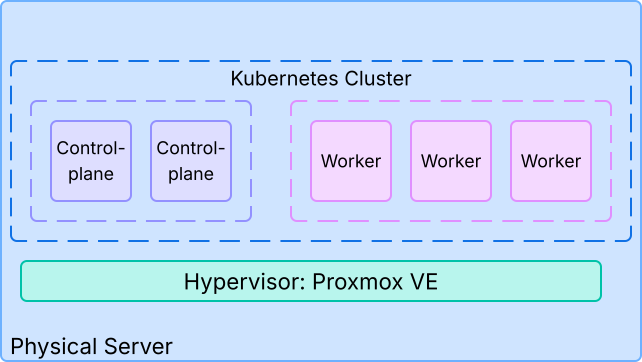
\includegraphics[width=0.7\textwidth]{k8s-cluster}
	\caption{Kubernetes cluster με δύο \textit{controlplane} κόμβους και τρεις
	\textit{κόμβους}} \label{fig:k8s-cluster}
\end{figure}

\subsection{Αυτοματισμοί υποδομής και διακυβέρνηση}

Όλα τα στοιχεία της πλατφόρμας ορίζονται δηλωτικά, με \textit{Helm charts} και
manifests που αποθηκεύονται σε κεντρικό αποθετήριο. Οι αλλαγές εφαρμόζονται
μέσω τυπικών ροών \textit{GitOps}: κάθε commit που επιφέρει αλλαγές στην υποδομή
<<ειδοποιεί>> έμμεσα έναν \textit{controller}, ο οποίος παρακολουθεί το
repository και συγχρονίζει την επιθυμητή κατάσταση με την τρέχουσα κατάσταση
του \textit{cluster}. Η πρακτική αυτή εξασφαλίζει ότι το \textit{production cluster}
αποτελεί ακριβές στιγμιότυπο του δηλωτικού μοντέλου, διευκολύνοντας την
auditability και την αναπαραγωγή σφαλμάτων.

Σε επίπεδο ασφάλειας, η πλατφόρμα οργανώνεται σε διακριτά \textit{Namespaces}
με αντίστοιχους κανόνες \textit{RBAC}, ώστε κάθε συνιστώσα να λειτουργεί εντός
περιορισμένου επιχειρησιακού πλαισίου. Η λογική αυτή ακολουθεί την καθιερωμένη
αρχή του «ελάχιστου απαιτούμενου δικαιώματος» και επιτρέπει στις υπηρεσίες να
εκτελούν μόνο τις λειτουργίες που τους αναλογούν, χωρίς να αποκτούν πρόσβαση σε
μη σχετιζόμενα υποσυστήματα. Η απομόνωση αυτή αποτελεί ικανοποιητικό επίπεδο
προστασίας για το scope της παρούσας εργασίας και διατηρεί τις υπηρεσίες πλήρως
ανεξάρτητες σε ό,τι αφορά την ανάπτυξη, τη συντήρηση και την παρακολούθησή
τους.

\section{Ροή δεδομένων σε πραγματικό χρόνο}

\subsection{Πηγές ροής δεδομένων}

Η αξιόπιστη και χαμηλής καθυστέρησης επεξεργασία ροών δεδομένων σε περιβάλλοντα
γεωργίας ακρίβειας προϋποθέτει τη διαχείριση ετερογενών πηγών, από θερμόμετρα
εδάφους έως αισθητήρες υγρασίας και \textit{pH}. Κάθε συσκευή εκτελεί το δικό
της ελαφρύ πρόγραμμα τηλεμετρίας, το οποίο υποστηρίζει διαφορετικές συχνότητες
εκπομπής και μπορεί να ρυθμιστεί ανάλογα με τη λειτουργική ανάγκη του
παραγωγού. Η πλατφόρμα παρέχει στον αισθητήρα τα απαραίτητα διαπιστευτήρια και
τις παραμέτρους λειτουργίας του, συμπεριλαμβανομένης της επιθυμητής granularity
του μηνύματος (π.χ.\ ανά 5, 30 ή 120 δευτερόλεπτα), ώστε κάθε συσκευή να
αποστέλλει δεδομένα με τρόπο προσαρμοσμένο στο προφίλ καλλιέργειας και στο
διαθέσιμο δίκτυο. Τα μηνύματα αποστέλλονται σε μορφή JSON μέσω \textit{MQTT}
και φτάνουν στο ingestion layer της πλατφόρμας με τη μορφή που τα εκπέμπει η
συσκευή, χωρίς ενδιάμεση τροποποίηση. Από εκεί και πέρα η ροή δεδομένων
δρομολογείται προς τα κατάλληλα topics και pipelines για περαιτέρω επεξεργασία,
όπως περιγράφεται στις επόμενες υποενότητες.

\subsection{Τεχνολογίες Streaming}

Στην προηγούμενη ενότητα παρουσιάστηκε το \textit{Apache Kafka} ως το βασικό
μέσο ενδιάμεσης επικοινωνίας μεταξύ των στοιχείων της πλατφόρμας. Σενάρια
\textit{streaming}, όπως αυτό της πλατφόρμας \textit{Nostradamus}, βασίζονται
στο \textit{Kafka} ως τον κεντρικό κόμβο του συστήματος, ο οποίος λειτουργεί ως
η κύρια <<πηγή αλήθειας>> για όλα τα υποσυστήματα. Κάθε γεγονός που συμβαίνει
στο σύστημα καταγράφεται αρχικά στο \textit{Kafka}, και στη συνέχεια κάθε
μικροϋπηρεσία εγγράφεται στο αντίστοιχο <<θέμα>> (\textit{topic}) ώστε να
λαμβάνει μόνο τα μηνύματα που της είναι απαραίτητα. Με αυτόν τον τρόπο
επιτυγχάνεται ο σαφής διαχωρισμός ανάμεσα στη ροή δεδομένων σε πραγματικό χρόνο
και στην κατανάλωση των μηνυμάτων. Συνεπώς, η σωστή σχεδίαση της υποδομής
συλλογής και μεταφοράς δεδομένων έως το \textit{Kafka} είναι κρίσιμη, καθώς από
εκεί και πέρα ο διαμοιρασμός τους στα υπόλοιπα υποσυστήματα γίνεται με απλό και
αποδοτικό τρόπο.

Για το \textit{deployment} του \textit{Kafka} στην πλατφόρμα επιλέχθηκε το
μοτίβο του \textit{Kubernetes Operator}, με στόχο την υψηλή διαθεσιμότητα, την
ανθεκτικότητα σε αστοχίες και την αυτοματοποιημένη διαχείριση του κύκλου ζωής
του συστήματος. Συγκεκριμένα, χρησιμοποιήθηκε ο \textit{Strimzi Kafka
Operator}, ο οποίος παρέχει πλήρη αυτοματοποίηση στην εγκατάσταση, ρύθμιση,
κλιμάκωση και αναβάθμιση των brokers, καθώς και στη διαχείριση των
\textit{topics} και των \textit{users}. Με αυτόν τον τρόπο αξιοποιούνται τα
πλεονεκτήματα του Kubernetes, όπως η ευκολία κλιμάκωσης, η αυτόματη
αποκατάσταση υπηρεσιών και η συνεπής διαχείριση πόρων, εξασφαλίζοντας παράλληλα
σταθερή και αποδοτική λειτουργία της υποδομής ροών. Τέλος, ο \textit{operator}
αυτός επιτρέπει την διαχείριση της υποδομής του \textit{Kafka} μέσω
\textit{GitOps} πρακτικών, γεγονός που ευθυγραμμίζεται με τις υπόλοιπες αρχές
και πρότυπα σχεδίασης της παρούσας εργασίας.

Είναι πλέον καθιερωμένη πρακτική οι αισθητήρες και γενικότερα οι χαμηλής
κατανάλωσης μικροελεγκτές που χρησιμοποιούνται σε υποδομές \textit{IoT} να
αποστέλλουν τα μηνύματά τους μέσω του πρωτοκόλλου \textit{MQTT}, καθώς αυτό
εξοικονομεί ενέργεια και επιτρέπει αποδοτική μετάδοση δεδομένων. Για την
εισαγωγή των μηνυμάτων αυτής της μορφής στο \textit{Kafka} απαιτείται η ύπαρξη
μηχανισμού γεφύρωσης. Στο πλαίσιο αυτό, αξιοποιήθηκε αρχικά το \textit{Strimzi
MQTT bridge}.

Ωστόσο, η ενσωματωμένη υλοποίηση του \textit{Strimzi} δεν υποστηρίζει ασφαλή
μεταφορά μέσω \textit{MQTTs}, γεγονός που αποτελεί κρίσιμο ζήτημα για την
παρούσα πλατφόρμα, δεδομένου ότι οι αισθητήρες βρίσκονται σε εξωτερικά δίκτυα.
Για την επίλυση του προβλήματος, ενσωματώθηκε ένας \textit{EMQX broker}, ο
οποίος λειτουργεί ως ασφαλής πύλη (\textit{secure gateway}) μεταξύ των
εξωτερικών συσκευών και του \textit{Kafka}, παρέχοντας υποστήριξη για
κρυπτογράφηση και μηχανισμούς πιστοποίησης σύμφωνα με τις απαιτήσεις της
αρχιτεκτονικής. Παράλληλα, ο \textit{EMQX broker} παρέχει δυνατότητες
φιλτραρίσματος βάσει των εισερχόμενων \textit{MQTT topics} και αντιστοίχισης
(\textit{mapping}) αυτών σε \textit{Kafka topics}, ώστε να προωθούνται στο
\textit{Kafka} μόνο τα απαραίτητα μηνύματα και να διατηρείται συνεπής η
ονοματολογία και η δομή των θεμάτων στην πλατφόρμα.

Η επιλογή του Kafka ως κεντρικού μηχανισμού μεταφοράς δεδομένων δικαιολογείται
και από τη φύση των γεωργικών συστημάτων, όπου παρατηρείται συχνά συνδυασμός
διαλείπουσας συνδεσιμότητας, απότομων αλλαγών στον ρυθμό παραγωγής δεδομένων
και ανομοιογενών payloads. Η εγγυημένη σειρά παράδοσης και η ανθεκτικότητα του
commit log καθιστούν το Kafka τον πλέον κατάλληλο μηχανισμό για ροές που
απαιτούν επαναληψιμότητα και ανοχή σε αστοχίες, ανεξαρτήτως του backend που
καταναλώνει τα μηνύματα.

\section{Προσωρινή αποθήκευση και cache drivers}

\subsection{Αρχιτεκτονική και ενσωμάτωση}

Το επίπεδο προσωρινής αποθήκευσης υιοθετεί το πρότυπο \textit{cache-aside}, με
αυστηρά όρια χρόνου ζωής (TTL 120 δευτερολέπτων) και υλοποίηση ως διακριτή
διασύνδεση. Η επιλογή αυτή επιτρέπει την εναλλαγή υποστρωμάτων χωρίς αλλαγές
στον κώδικα της εφαρμογής, ενώ το ίδιο interface παρέχει ενιαία συλλογή
μετρικών και ιχνηλασιμότητα. Εκτός του \textit{Valkey}, έχουν δημιουργηθεί
adapters για \textit{Memcached} και \textit{Dragonfly}, τους οποίους η
πλατφόρμα ενεργοποιεί ακόμη και κατά τη διάρκεια πειραμάτων συγκριτικής
αξιολόγησης ή ως μηχανισμό εφεδρείας. Η ύπαρξη πολλαπλών drivers προσφέρει
επιχειρησιακή ευελιξία: σε περίπτωση που ένα υπόστρωμα προσωρινής αποθήκευσης
παρουσιάσει αυξημένη καθυστέρηση ή μειωμένη διαθεσιμότητα, ο controller
επιτρέπει την άμεση μετάβαση σε εναλλακτικό driver. Σε συνδυασμό με τις
\textit{readiness probes}, εξασφαλίζεται ότι οι διεπαφές των χρηστών όπως το
\textit{UI} και τα τρίτα συστήματα δεν βλέπουν ποτέ ασταθή κατάσταση.

\subsection{Επιλογή και συγκριτική αξιολόγηση υποστρωμάτων}

Η επιλογή των τριών επιμέρους υποστρωμάτων καθορίστηκε από κριτήρια
συμβατότητας, λειτουργικότητας και αναμενόμενης επίδοσης. Το \textit{Valkey}
υιοθετήθηκε ως αναφορά, καθώς αποτελεί την πλέον συμβατή και κοινοτικά
υποστηριζόμενη μετεξέλιξη του οικοσυστήματος Redis, με πλούσιο σύνολο δομών
δεδομένων και δυνατότητα scripting, στοιχεία απαραίτητα για μελλοντικές
λειτουργίες της πλατφόρμας. Το \textit{Dragonfly} επιλέχθηκε λόγω της
αρχιτεκτονικής του που εστιάζει στην ενιαία πολυνηματική αξιοποίηση της μνήμης
και στο περιορισμένο αποτύπωμα πόρων, ενώ διατηρεί συμβατότητα σε επίπεδο
πρωτοκόλλου με το Valkey/Redis, καθιστώντας την εναλλαγή πρακτικά διαφανή.
Τέλος, το \textit{Memcached} ενσωματώθηκε ως ελαφριά, εδραιωμένη λύση με
περιορισμένο σύνολο λειτουργιών, η οποία όμως προσφέρει προβλέψιμη καθυστέρηση,
καθιστώντας την ιδανικό σημείο αναφοράς για συγκρίσεις καθαρού ρυθμού
διεκπεραίωσης.

Σημαντική παράμετρος της μελέτης είναι ότι το \textit{Valkey} και το
\textit{Dragonfly} μοιράζονται κοινό πρωτόκολλο και μοντέλο δεδομένων, γεγονός
που επιτρέπει την αξιολόγησή τους ως εναλλακτικές υλοποιήσεις της ίδιας λογικής
διασύνδεσης. Και τα δύο υποστρώματα παρέχουν μονόκλωνη σημασιολογία εκτέλεσης
εντολών, υποστηρίζουν scripting και σύνθετες δομές (δομές κατακερματισμού,
ταξινομημένα σύνολα), καθώς και χαρακτηριστικά όπως replication και μονιμότητα
δεδομένων. Κατά συνέπεια, τυχόν διαφοροποιήσεις στην επίδοση μπορούν να
αποδοθούν αποκλειστικά στην εσωτερική μηχανική υλοποίηση (μηχανή
κατακερματισμού, χρονοδρομολογητής, στρατηγικές χρήσης μνήμης) και όχι σε
αλλαγές του προγραμματιστικού μοντέλου. Η επιλογή τους επιτρέπει, επομένως, τη
συγκριτική απομόνωση των πλεονεκτημάτων που φέρει μια πιο επιθετική
πολυνηματική προσέγγιση (\textit{Dragonfly}) έναντι της κλασικής, πλήρως
συμβατής ερμηνείας (\textit{Valkey}), χωρίς να απαιτείται προσαρμογή του
εφαρμοστικού κώδικα.

\subsection{Πειραματικές υποθέσεις}

Πριν από την πειραματική διαδικασία διατυπώθηκαν συγκεκριμένα υποθετικά
σενάρια: αναμενόταν ότι το \textit{Memcached}, χάρη στο απλούστερο δυαδικό
πρωτόκολλο και την απουσία σύνθετων δομών, θα υπερτερεί σε P95 καθυστέρηση
ανάγνωσης και εγγραφής όταν το φορτίο είναι πλήρως συμμετρικό. Αντίστοιχα, η
υπόθεση για το \textit{Valkey} ήταν ότι θα εμφανίσει υψηλότερη σταθερότητα υπό
παρατεταμένα φορτία και καλύτερη συμπεριφορά σε σενάρια με ανάγκη αδιαίρετων
λειτουργιών. Για το \textit{Dragonfly}, η αναμενόμενη συμπεριφορά τοποθετήθηκε
ενδιάμεσα: στόχος ήταν να επαληθευθεί αν ο πολυνηματικός χρονοδρομολογητής και
η διαχείριση μνήμης που διαθέτει οδηγούν σε ρυθμό διεκπεραίωσης συγκρίσιμο με
το \textit{Memcached}, διατηρώντας παράλληλα τη λειτουργική πληρότητα του
\textit{Valkey}. Οι υποθέσεις αυτές καταγράφονται εδώ προκειμένου να
συσχετιστούν στη συνέχεια με τα αποτελέσματα του
Κεφαλαίου~\ref{chap:experiments}.

Η διατύπωση των παραπάνω υποθέσεων δεν στοχεύει απλώς στη σύγκριση διαφορετικών
υλοποιήσεων, αλλά και στην αξιολόγηση του κατά πόσο η πλατφόρμα μπορεί να
υποστηρίξει ετερογενείς drivers χωρίς αλλαγές στην επιχειρησιακή λογική. Η
προσέγγιση αυτή επιτρέπει τον διαχωρισμό της λειτουργικότητας της εφαρμογής από
τις επιδόσεις του υποστρώματος, στοιχείο που αποτελεί κρίσιμο παράγοντα για την
επεκτασιμότητα της πλατφόρμας σε μελλοντικά περιβάλλοντα και διαφορετικά
workloads.

\subsection{Στρατηγικές caching}

Η υιοθέτηση μηχανισμών κρυφής μνήμης σε κατανεμημένα συστήματα συνοδεύεται από
διαφορετικά πρότυπα (\textit{patterns}) υλοποίησης, καθένα από τα οποία φέρει
πλεονεκτήματα και περιορισμούς. Τα συνηθέστερα είναι τα ακόλουθα:

\subsubsection{Read-through}

Στο πρότυπο αυτό, όλες οι αναγνώσεις δεδομένων γίνονται μέσω της cache. Σε
περίπτωση που το ζητούμενο κλειδί δεν υπάρχει, η ίδια η cache αναλαμβάνει να
ανακτήσει τα δεδομένα από τη βάση και να τα αποθηκεύσει πριν τα επιστρέψει στον
χρήστη. Το πλεονέκτημα είναι η απλοποίηση της εφαρμογής, καθώς η λογική
ανάκτησης μετατίθεται στο cache layer. Ωστόσο, απαιτείται στενή ενσωμάτωση της
cache με τη βάση, κάτι που δυσχεραίνει την παραμετροποίηση σε περιβάλλοντα με
ετερογενείς πηγές δεδομένων.

\subsubsection{Write-through}

Σε αυτήν τη στρατηγική, κάθε εγγραφή περνάει πρώτα από την cache και στη
συνέχεια στη βάση δεδομένων. Η μέθοδος αυτή εξασφαλίζει συνεπή δεδομένα, καθώς
cache και βάση ενημερώνονται ταυτόχρονα, αλλά αυξάνει τον χρόνο απόκρισης για
κάθε write. Επιπλέον, το συνολικό throughput περιορίζεται από τον πιο αδύναμο
(αργό) κρίκο της αλυσίδας.

\subsubsection{Write-behind (ή Write-back)}

Τα δεδομένα γράφονται αρχικά μόνο στην cache και σε δεύτερο χρόνο, με ασύγχρονο
τρόπο, προωθούνται στη βάση. Το σχήμα αυτό προσφέρει υψηλές επιδόσεις για
σενάρια έντονου write load, αλλά εισάγει κινδύνους απώλειας δεδομένων σε
περίπτωση αστοχίας της cache, ενώ η βάση ενδέχεται να μην αντικατοπτρίζει την
πιο πρόσφατη κατάσταση.

\subsubsection{Cache-aside (ή Lazy loading)}

Στο πρότυπο αυτό, η εφαρμογή ελέγχει πρώτα την cache. Αν τα δεδομένα υπάρχουν,
επιστρέφονται άμεσα. Αν όχι, η εφαρμογή ανατρέχει στη βάση δεδομένων,
επιστρέφει τα αποτελέσματα στον χρήστη και ταυτόχρονα τα εισάγει εκ νέου στην
cache για μελλοντική χρήση. Το κύριο πλεονέκτημα είναι η απλότητα: η cache
λειτουργεί ως προαιρετικό επιταχυντικό στρώμα, χωρίς να απαιτείται βαθιά
ενσωμάτωση με τη βάση δεδομένων. Το μειονέκτημα είναι ότι τα δεδομένα μπορεί να
είναι στιγμιαία \textit{stale}, ειδικά σε περιπτώσεις έντονων ενημερώσεων.

\medskip Για τις ανάγκες της παρούσας πλατφόρμας, επιλέχθηκε το πρότυπο
\textit{cache-aside}, καθώς τα ερωτήματα αφορούν κυρίως αναγνώσεις πρόσφατων
τιμών αισθητήρων με χαμηλή πιθανότητα συνεχών τροποποιήσεων. Με τον τρόπο αυτό,
η ScyllaDB παραμένει η πηγή αλήθειας (\textit{source of truth}), ενώ το Valkey
cluster χρησιμοποιείται για να μειώσει τον χρόνο απόκρισης σε συχνά αιτήματα,
επιτυγχάνοντας ισορροπία ανάμεσα σε απόδοση και συνέπεια.

\section{Επίπεδο υπηρεσιών και εφαρμογής}

Το επίπεδο υπηρεσιών συγκροτείται γύρω από ένα κεντρικό API gateway, το οποίο
αποτελεί τη βασική διεπαφή των χρηστών και των downstream συστημάτων με τα
στοιχεία της πλατφόρμας. Η σχεδίασή του ακολουθεί modular αρχιτεκτονική, με
σαφή διαχωρισμό ευθυνών ανάμεσα στη διαχείριση πόρων, την επεξεργασία ροών, την
προσωρινή αποθήκευση και την παρατηρησιμότητα.

\subsection{Valkey cluster}

Η υποστήριξη του μηχανισμού cache υλοποιείται με \textit{Valkey cluster}, ο
οποίος αναπτύχθηκε μέσω του \textit{Hyperspike Operator}. Η λύση αυτή
εξασφαλίζει οριζόντια κλιμάκωση και υψηλή διαθεσιμότητα σε περιβάλλον
Kubernetes, με αυτοματοποιημένη διαχείριση των κόμβων Redis/Valkey.

Συνδυάζοντας τον Valkey cluster για ταχύτατη εξυπηρέτηση πρόσφατων μετρήσεων με
τη ScyllaDB για ανθεκτική και αναλυτική αποθήκευση, η πλατφόρμα διατηρεί
ισορροπία ανάμεσα σε χαμηλή καθυστέρηση και αξιοπιστία δεδομένων.

\begin{figure}[H]
	\centering
	\includegraphics[width=0.7\textwidth]{cache-aside}
	\caption{Λογικό διάγραμμα του προτύπου \textit{cache-aside}:
		το API ελέγχει αρχικά την κρυφή μνήμη (Valkey) για την αναζήτηση
		δεδομένων και, σε περίπτωση αποτυχίας, προσφεύγει στη ScyllaDB.
		Τα δεδομένα επιστρέφονται στον χρήστη και ταυτόχρονα επανεισάγονται
		στην cache, ώστε να εξυπηρετηθούν με χαμηλή καθυστέρηση σε επόμενα
		αιτήματα.}
	\label{fig:cache-aside-diagram}
\end{figure}

\subsection{API gateway και διαχείριση πόρων}

Το API παρέχει REST endpoints για την εγγραφή αγροτεμαχίων, την ενεργοποίηση
αισθητήρων, την έκδοση διαπιστευτηρίων και την προβολή συγκεντρωτικών τιμών
μέσω του \texttt{/aggregate}. Το API ελέγχει τα δικαιώματα κάθε κλήσης,
χαρτογραφεί τα αιτήματα σε συγκεκριμένα pipelines και επιβάλλει πολιτικές που
προκύπτουν από την ανάλυση των επιχειρησιακών ροών.

Η αρχιτεκτονική του API στηρίζεται σε διακριτά πακέτα: ένα για την πρόσβαση στη
βάση \textit{Scylla}, ένα για το caching layer, ένα για τη δρομολόγηση
αιτημάτων, καθώς και βοηθητικές βιβλιοθήκες για serialization, logging και
ιχνηλασιμότητα. Η επικοινωνία με τη Scylla υλοποιείται μέσω του οδηγού
\texttt{gocql}, ενώ το caching layer υλοποιείται ως ανεξάρτητο module
αποσυνδεδεμένο από τον αποθηκευτικό μηχανισμό.

\subsection{Διαχείριση Arroyo pipelines}

Η πλατφόρμα \textit{Arroyo} χρησιμοποιείται ως βασικό στοιχείο του streaming
layer, καθώς παρέχει connectors από \textit{Kafka} προς \textit{Scylla} σε
λειτουργία συνεχούς επεξεργασίας. Το API οργανώνει τα \textit{pipelines}
χρησιμοποιώντας abstractions που αντιστοιχούν σε αγροτεμάχια και αισθητήρες.
Μόλις καταχωρηθεί μία νέα συσκευή ή καταφτάσουν δεδομένα, ο controller
δημιουργεί δυναμικά το αντίστοιχο Arroyo job, το συνδέει με το κατάλληλο
\textit{topic} και παρακολουθεί το throughput του. Αν ένα job τερματιστεί, η
υπηρεσία αναλαμβάνει την αυτόματη επανεκκίνησή του και την ενημέρωση των
καταναλωτών, εξασφαλίζοντας \textit{self-healing} συμπεριφορά πέρα από τα όρια
του Kubernetes.

Παρότι σήμερα το Arroyo αξιοποιείται κυρίως ως connector, η σχεδίαση του API
επιτρέπει τη μελλοντική έκθεση επιπλέον λειτουργιών σε προχωρημένους χρήστες ή
σε DSL που θα πατήσει στο ίδιο API. Με αυτόν τον τρόπο ο κεντρικός έλεγχος
παραμένει στους developers της πλατφόρμας, αλλά παρέχεται σαφές σημείο
επέκτασης για πιο πολύπλοκα υπολογιστικά pipelines.

\subsection{Ανθεκτικότητα και ανοχή σε σφάλματα}

Στο API λειτουργούν controllers (υλοποιημένοι ως goroutines), οι οποίοι:

\begin{itemize}
	\item παρακολουθούν τις καταστάσεις των Arroyo jobs,
	\item αναδημιουργούν pipelines όταν απαιτείται,
    	\item συγχρονίζουν connectors μεταξύ Kafka και Scylla,
    	\item διασφαλίζουν ότι καμία ροή δεν μένει ανεπεξέργαστη.
\end{itemize}

Με αυτόν τον τρόπο η υπηρεσία επιτυγχάνει self-healing συμπεριφορά, η οποία
υπερβαίνει την αυτόματη αποκατάσταση που προσφέρει το Kubernetes.

\subsection{Υπηρεσία \textit{/aggregate} και caching layer}

Η προβολή συγκεντρωτικών μετρήσεων αποτελεί αναπόσπαστο κομμάτι κάθε συστήματος
που επεξεργάζεται δεδομένα αισθητήρων σε πραγματικό χρόνο. Παρότι η πλατφόρμα
διατηρεί αναλυτική ροή μέσω των pipelines, οι περισσότεροι παραγωγοί και
εφαρμογές καταναλώνουν τα δεδομένα σε συνοπτική μορφή, σε παράθυρα
συγκεκριμένης διάρκειας και για συγκεκριμένο τύπο αισθητήρα. Για τον λόγο αυτόν
σχεδιάστηκε η υπηρεσία \textit{/aggregate}, η οποία λειτουργεί ως ενιαίο σημείο
πρόσβασης για την εξαγωγή απλοποιημένων στατιστικών (π.χ.\ ελάχιστο, μέγιστο,
μέσο όρο) πάνω σε πρόσφατα δεδομένα. Η υπηρεσία αυτή αναλαμβάνει να
εξυπηρετήσει τα πιο συχνά αναγνώσιμα workloads της πλατφόρμας με προβλέψιμο
latency, αξιοποιώντας το caching layer και τις μετρικές παρατηρησιμότητας που
έχουν ενσωματωθεί. Κάθε κλήση δέχεται παραμέτρους παραθύρου (π.χ. 1 ώρα) και
τύπο αισθητήρα (θερμοκρασία, υγρασία, \textit{pH}), επιστρέφοντας ταυτόχρονα
\textit{min}, \textit{max} και \textit{average} τιμές. Η υλοποίηση ακολουθεί
μοτίβο \textit{cache-aside}: αρχικά επιχειρείται \textit{CacheFetch}, στη
συνέχεια γίνεται \textit{DBFetch} από τη \textit{Scylla} μόνο αν υπάρξει
\textit{miss}, και τέλος τα αποτελέσματα αποθηκεύονται με TTL 120
δευτερολέπτων. Ο κύκλος αυτός είναι πλήρως ορατός μέσω traces, ενώ οι σχετικές
μετρικές τροφοδοτούν τα dashboards που χρησιμοποιήθηκαν και στα πειράματα.

Το caching layer είναι ανεξάρτητη βιβλιοθήκη με κοινό interface, στην οποία
έχουν αναπτυχθεί drivers για \textit{Valkey}, \textit{Memcached} και
\textit{Dragonfly}. Ο εκάστοτε driver επιλέγεται με παραμετροποίηση στο
\textit{deployment}, γεγονός που επέτρεψε τη γρήγορη εκτέλεση των benchmark
σεναρίων και την ανάλυση των P95 καθυστερήσεων. Παράλληλα, ο ίδιος μηχανισμός
καταγράφει \textit{cache hit/miss} με granularity ανά αισθητήρα και είδος
aggregation, επιτρέποντας την αξιολόγηση της αποδοτικότητας του caching ανά
workload. Ως μελλοντική βελτίωση σχεδιάζεται ένα ταχύτερο endpoint μεταφοράς
δεδομένων μεταξύ υπηρεσιών, ώστε να παρακάμπτει πλήρως το UI όταν απαιτείται
ενδοσυστημική ολοκλήρωση.

Η συγκεκριμένη υπηρεσία λειτουργεί, επιπλέον, ως αντιπροσωπευτικό υπόδειγμα του
συνολικού τρόπου με τον οποίο η πλατφόρμα χειρίζεται δεδομένα αισθητήρων. Το
\textit{/aggregate} προσφέρει ένα πλήρως λειτουργικό σημείο δοκιμής για το
caching layer, καθιστώντας εφικτή την αξιολόγηση διαφορετικών drivers και τη
μέτρηση της συμπεριφοράς τους κάτω από πραγματικό φόρτο. Ως εκ τούτου, η
υπηρεσία διαδραματίζει διττό ρόλο: από τη μία επιτρέπει την άμεση κατανάλωση
συγκεντρωτικών μετρήσεων από τους παραγωγούς, και από την άλλη παρέχει ένα
σταθερό και επαναλήψιμο περιβάλλον για benchmarking, debugging και ανάλυση των
επιδόσεων της υποδομής. Παρότι το \textit{/aggregate} καλύπτει τις βασικές
ανάγκες του τρέχοντος συστήματος, η υφιστάμενη αρχιτεκτονική επιτρέπει τη
δημιουργία επιπλέον endpoints με παρόμοια λογική, είτε για πιο σύνθετες
αναλύσεις είτε για επέκταση σε νέα είδη αισθητήρων και νέους τύπους χρονικών
ερωτημάτων, μετατρέποντας σταδιακά την πλατφόρμα σε πλήρες εργαλείο προβολής
και επεξεργασίας γεωργικών δεδομένων σε πραγματικό χρόνο.

\subsection{Frontend και διεπαφές παρακολούθησης}

Παρότι το κύριο βάρος της εργασίας εστιάζει στα υποσυστήματα υποδομής,
επεξεργασίας ροών και προσωρινής αποθήκευσης, η ύπαρξη ενός λειτουργικού
frontend κρίθηκε απαραίτητη ώστε να αναδεικνύονται στην πράξη οι δυνατότητες
του API και του caching layer. Το frontend λειτουργεί ως το πρώτο σημείο επαφής
των παραγωγών με την πλατφόρμα και αποτελεί ένα ελαφρύ, πλήρως λειτουργικό
παράδειγμα κατανάλωσης των υπηρεσιών που περιγράφηκαν στις προηγούμενες
ενότητες. Πρακτικά, χρησιμεύει ως «βιτρίνα» της αρχιτεκτονικής: επιτρέπει την
ορατή επαλήθευση της ροής δεδομένων, της συμπεριφοράς του \textit{/aggregate}
και της απόδοσης του caching layer, χωρίς να απαιτούνται ειδικά εργαλεία ή
σύνθετα dashboard setups.

Το UI καταναλώνει το API gateway και παρέχει φόρμες για την εγγραφή
αγροτεμαχίων, την ενεργοποίηση αισθητήρων και την διαχείριση των ρυθμίσεών
τους. Εμφανίζει επίσης τις πιο πρόσφατες μετρήσεις ανά σημείο, αξιοποιώντας
άμεσα τα αποτελέσματα της υπηρεσίας \textit{/aggregate}. Με αυτόν τον τρόπο το
frontend λειτουργεί και ως δείκτης ορθής λειτουργίας του caching layer, αφού η
διαφορά μεταξύ cache hits και misses αποτυπώνεται άμεσα στον χρόνο απόκρισης
του UI.

Πέρα από τις βασικές ροές onboarding, το frontend παρέχει συνοπτικές μετρικές
που συνοψίζουν την τρέχουσα κατάσταση του αγρού, επιτρέποντας στον χρήστη να
λάβει μια γρήγορη εικόνα της δραστηριότητας των αισθητήρων. Για πιο αναλυτικά
KPIs, χρονοσειρές και διαγνωστικά στοιχεία, οι χρήστες ανακατευθύνονται στα
εξειδικευμένα Grafana boards, όπου συγκεντρώνονται οι μετρικές από το
monitoring stack της πλατφόρμας.

Ο σχεδιασμός του frontend κρατήθηκε εσκεμμένα απλός. Στόχος του δεν είναι να
αναπαράγει την πληρότητα ενός παραγωγικού dashboard, αλλά να λειτουργήσει ως
reference implementation πάνω στο API, διευκολύνοντας την ανάπτυξη νέων
υπηρεσιών και αποτελώντας σημείο εκκίνησης για μελλοντικές επεκτάσεις. Η
υφιστάμενη δομή επιτρέπει την προσθήκη πρόσθετων σελίδων και endpoints, από
εμπλουτισμένα γραφήματα μέχρι real-time feeds, χωρίς να απαιτούνται αλλαγές στο
υπόβαθρο της πλατφόρμας.

\section{Παρατηρησιμότητα}

Η παρατηρησιμότητα αποτελεί θεμελιώδες χαρακτηριστικό της πλατφόρμας, καθώς
επιτρέπει την πλήρη κατανόηση της συμπεριφοράς του συστήματος και την
επαλήθευση ότι η ροή των αισθητήριων δεδομένων λειτουργεί όπως αναμένεται. Η
παρούσα ενότητα αναλύει τους τρεις βασικούς άξονες παρατηρησιμότητας που
υλοποιήθηκαν: \textit{μετρικές}, \textit{καταγραφές} και
\textit{ιχνηλασιμότητα}.

\subsection{Μετρικές και SLI παρακολούθησης}

Η προσέγγιση με \textbf{προτεραιότητα στην παρατηρησιμότητα} ακολουθείται σε
όλα τα στοιχεία του συστήματος, ώστε η ροή των αισθητήριων δεδομένων να είναι
πλήρως μετρήσιμη και επαληθεύσιμη. Τα βασικά \textit{SLI} που παρακολουθούνται
είναι η καθυστέρηση ανάγνωσης και εγγραφής στην cache, ο δείκτης \textit{cache
miss} και ο χρόνος ανάγνωσης της βάσης \textit{Scylla}. Τα μεγέθη αυτά
εκτίθενται από τις υπηρεσίες μέσω \textit{Prometheus exporters} και
προβάλλονται σε ενιαία \textit{Grafana dashboards}, επιτρέποντας άμεση σύγκριση
μεταξύ διαφορετικών cache drivers ή διαφορετικών pipelines.

Η συλλογή σημάτων δεν περιορίζεται σε επίπεδο υποδομής. Κάθε κριτικό σημείο της
υπηρεσίας \textit{/aggregate} φέρει στοχευμένα \textit{metrics}, όπως ο χρόνος
ολοκλήρωσης των λειτουργιών \textit{CacheFetch}, \textit{DBFetch} και
\textit{CacheStore}, καθώς και αντιστοιχίσεις με το παράθυρο (π.χ. 15 λεπτά, 1
ώρα) και το είδος αισθητήρα (θερμοκρασία, υγρασία, pH). Με αυτόν τον τρόπο η
παρατηρησιμότητα διασταυρώνεται με το \textit{business logic} της πλατφόρμας
και τα πειραματικά αποτελέσματα μπορούν να χαρτογραφηθούν άμεσα σε συγκεκριμένα
workloads.

Η δυνατότητα συσχέτισης σημάτων από πολλαπλά επίπεδα, όπως ο χρόνος ανάγνωσης
cache, η καθυστέρηση επεξεργασίας στους brokers και ο τελικός χρόνος απόκρισης
του API, προσδίδει στην πλατφόρμα χαρακτηριστικά cross-layer παρατηρησιμότητας.
Τα συνδυαστικά αυτά σήματα διευκολύνουν την αναγνώριση συστημικών προβλημάτων
που δεν είναι εμφανή όταν μετρώνται απομονωμένα, όπως συμφόρηση I/O ή μη
ομοιόμορφη κατανομή φορτίου σε πυρήνες.

\subsection{Καταγραφές και διασταύρωση συμβάντων}

Πέρα από τις μετρικές, εφαρμόζεται τυποποιημένο σύστημα καταγραφής
(\textit{structured logging}) με εμπλουτισμό μεταδεδομένων και
\textit{correlation IDs}. Όλα τα logs ρέουν προς \textit{Grafana Loki},
επιτρέποντας πολυδιάστατη αναζήτηση ανά αισθητήρα, pipeline ή χρήστη. Η
διάσταση της ιχνηλασιμότητας αναλύεται εκτενώς στην υποενότητα «Ιχνηλασιμότητα
και ανάλυση αιτημάτων», όπου περιγράφεται ο τρόπος με τον οποίο τα traces
συμπληρώνουν τα παραπάνω σήματα.

Το σύστημα καταγραφής λειτουργεί συμπληρωματικά προς τις μετρικές: σε
περιπτώσεις απόκλισης χρόνου απόκρισης, τα logs παρέχουν το πλαίσιο (context)
και τα συμβάντα που οδήγησαν στη συγκεκριμένη συμπεριφορά.

\subsection{Ιχνηλασιμότητα και ανάλυση αιτημάτων}

Η πλήρης ιχνηλασιμότητα (\textit{tracing}) αποτελεί τον τρίτο πυλώνα της
παρατηρησιμότητας και επιτρέπει την αποσύνθεση κάθε αιτήματος σε επιμέρους
λειτουργικές φάσεις. Για τον σκοπό αυτόν χρησιμοποιήθηκε η βιβλιοθήκη
\textit{OpenTelemetry}, με δρομολόγηση των traces στην υπηρεσία \textit{Tempo}
του Grafana μέσω ενός \textit{OTLP gRPC} εξαγωγέα.

Η αρχικοποίηση του tracer provider γίνεται κατά την εκκίνηση της υπηρεσίας: ο
εξαγωγέας συνδέεται στο endpoint του Tempo, ενεργοποιείται ο batch processor
για αποδοτική αποστολή παρτίδων και ορίζεται \textit{resource} με
χαρακτηριστικά όπως το όνομα υπηρεσίας (\textit{nostradamus-api}). Η διαδικασία
αρχικοποίησης μεριμνά επίσης για την ασφαλή αποδέσμευση του tracer provider
κατά τον τερματισμό, ώστε να μη χαθούν spans που βρίσκονται σε εκκρεμότητα.

Σε επίπεδο εφαρμογής, κάθε κλήση στο \textιt{/aggregate} ξεκινά span με το
context του αιτήματος, επιτρέποντας την αλυσίδωση με downstream κλήσεις. Η
υπηρεσία καταγράφει χαρακτηριστικά που περιγράφουν τα βασικά query parameters
(αισθητήρας, παράθυρο, τύπος μετρήσεων) και αποτυπώνει την τελική κατάσταση με
βάση τους κωδικούς επιστροφής του \textit{OpenTelemetry} (π.χ. \textit{OK},
\textit{Error}). Τα σημεία ελέγχου που χειρίζονται σφάλματα παραμετρικών
ελέγχων ή επικοινωνίας με τη βάση δεδομένων συνοδεύουν το span με σχετικές
εγγραφές (\textit{recorded errors}) και εμπλουτισμένα logs, έτσι ώστε τα traces
να απεικονίζουν πλήρως το μονοπάτι που ακολουθήθηκε.

\subsubsection{Ιχνηλασιμότητα στο caching layer}

Ιδιαίτερη έμφαση δίνεται στην ενοποίηση της ιχνηλασιμότητας με το caching
layer. Κάθε driver (π.χ. \textit{Memcached}, \textit{Valkey}) δημιουργεί
δευτερεύοντα spans για τις λειτουργίες \textit{FetchAggregate} και
\textit{StoreAggregate}, μεταφέροντας το context του αρχικού HTTP αιτήματος. Τα
spans φέρουν κοινά attributes, όπως το είδος του driver, το cache key και τη
χρονική διάρκεια ζωής της εγγραφής. Επιπλέον, η ροή αποτυπώνει με σαφήνεια τα
αποτελέσματα (\textit{hit}, \textit{miss}, \textit{corrupt}) και όλες τις
συνθήκες σφάλματος, καθώς καταγράφονται μαζί με το αντίστοιχό τους status.

Έτσι, το τελικό trace απεικονίζει ολόκληρο το μονοπάτι CacheFetch $\rightarrow$
DBFetch $\rightarrow$ CacheStore, συμπεριλαμβανομένων των χρονικών μεγεθών που
παρακολουθούνται παράλληλα και από τα metrics.

\subsubsection{Πλεονεκτήματα της ενιαίας ιχνηλασιμότητας}

Η παραπάνω προσέγγιση έχει δύο σημαντικά πλεονεκτήματα. Πρώτον, επιτρέπει την
ταχεία συσχέτιση των χρονικών αποκλίσεων που εμφανίζονται στα dashboards με
συγκεκριμένες κλήσεις και παραμέτρους, γεγονός κρίσιμο για την κατανόηση των
P95 καθυστερήσεων. Δεύτερον, παρέχει πλήρη ορατότητα στο σύστημα cache-aside,
προσφέροντας στοιχεία για τη συμπεριφορά κάθε driver χωρίς να απαιτείται
ξεχωριστή υλοποίηση debugging.

Σε ευρύτερο πλαίσιο, η ιχνηλασιμότητα αποτελεί βασικό μηχανισμό αποσφαλμάτωσης
σε κατανεμημένα περιβάλλοντα, όπου οι πιθανές αιτίες καθυστέρησης δεν
εντοπίζονται σε μία μόνο διεργασία αλλά προκύπτουν από την αλληλεπίδραση
πολλαπλών μικροϋπηρεσιών. Η δυνατότητα οπτικοποίησης των spans επιτρέπει την
κατανόηση του πραγματικού data path και καθιστά εφικτή την απομόνωση αιχμών
καθυστέρησης που συνήθως καλύπτονται από αθροιστικές μετρικές.

\section{Ένταξη πελάτη}

Η διαδικασία onboarding λαμβάνει χώρα αποκλειστικά μέσω του API gateway. Αρχικά
ο παραγωγός καταχωρεί τα στοιχεία του αγροτεμαχίου και των αισθητήρων, ενώ
έπειτα μπορεί να λάβει τα διαπιστευτήρια του κάθε αισθητήρα. Στη συνέχεια, το
API δημιουργεί τα αντίστοιχα topics στο \textit{Kafka}, συνδέει το αγροτεμάχιο
με το κατάλληλο Arroyo pipeline και ενεργοποιεί τη ροή δεδομένων. Τέλος, το
caching layer ενημερώνει τα indices ώστε τα πρόσφατα δεδομένα να είναι
διαθέσιμα αμέσως στο UI.

\begin{figure}[H] \centering
	\includegraphics[width=0.7\textwidth]{client-onboarding-process}
	\caption{Διάγραμα δραστηριότητας για τη διαδικασία ένταξης νέου πελάτη}
	\label{fig:client-onboarding-activity}
\end{figure}


\chapter{Πειράματα}
\label{chap:experiments}

Η παρούσα ενότητα εξετάζει τη συμπεριφορά των μηχανισμών προσωρινής αποθήκευσης
που υποστηρίζουν το endpoint \textit{/aggregate}, το οποίο αποτελεί βασικό
συστατικό της πλατφόρμας \textit{Nostradamus}. Η υπηρεσία αυτή υλοποιεί
παραθυρικές συναθροίσεις σε χρονοσειρές αισθητήρων και λειτουργεί ως μεσαίο
επίπεδο μεταξύ της εφαρμογής και της μόνιμης βάσης δεδομένων. Η καθυστέρηση
ανάγνωσης και εγγραφής στο \textit{cache layer} μεταφέρεται άμεσα στον χρόνο
απόκρισης του \textit{API}, επομένως η απόδοση του εκάστοτε υποστρώματος
αποτελεί πρωτεύοντα παράγοντα για τη συνολική σταθερότητα της πλατφόρμας.

Πριν από την παρουσίαση των αποτελεσμάτων, αξίζει να σημειωθεί ότι το
\textit{/aggregate} είναι ιδιαίτερα ευαίσθητο σε καθυστερήσεις, επειδή κάθε
αίτημα ενεργοποιεί υπολογισμό παραθύρου με βάση πρόσφατες μετρήσεις αισθητήρων.
Το \textit{cache layer} δεν λειτουργεί ως συμπληρωματικό στοιχείο αλλά ως
κρίσιμο μέρος του χρόνου διαδρομής των αιτημάτων. Επομένως, ακόμη και μικρές
διαφορές στα \textit{percentiles} των καθυστερήσεων αντικατοπτρίζονται άμεσα
στη συνολική εμπειρία χρήσης και στη σταθερότητα της πλατφόρμας.

\section{Διατύπωση στόχου και κριτήρια αξιολόγησης}

Στόχος της πειραματικής διαδικασίας είναι η αποτίμηση της απόδοσης και της
σταθερότητας δύο πλήρως εναλλάξιμων cache drivers (\textit{Valkey},
\textit{Memcached}) όταν χρησιμοποιούνται από το \textit{/aggregate} υπό
συνθήκες συνεχούς φόρτου, όπως αυτές που προσομοιάζουν ένα αγροτικό
\textit{deployment}. Η αξιολόγηση επικεντρώνεται σε τρεις κρίσιμες παραμέτρους,
οι οποίες αντικατοπτρίζουν τις πραγματικές απαιτήσεις ενός συστήματος
\textit{IoT} με συνεχή ροή δεδομένων:

\begin{enumerate}
	\item \textbf{Απόδοση ανάγνωσης και εγγραφής ($\text{I/O}$ Latency)}.
		Εξετάζονται συμμετρικά τα μονοπάτια \textit{cache hit} και
		\textit{cache miss}, καθώς αμφότερα συνεισφέρουν στον τελικό
		χρόνο απόκρισης του endpoint \textit{/aggregate} και την
		αποφόρτιση της μόνιμης βάσης δεδομένων.
	\item \textbf{Σταθερότητα σε υψηλά percentiles (P95, P99)}. Για
		συστήματα πραγματικού χρόνου, η μέση τιμή (P50) είναι ανεπαρκής
		δείκτης. Τα υψηλά percentiles (P95 και άνω) είναι εκεί όπου
		εκδηλώνονται οι χρονικές αποκλίσεις (tail latencies) που
		επηρεάζουν ουσιαστικά την εμπειρία χρήστη και την
		προβλεψιμότητα του συστήματος.
	\item \textbf{Συμπεριφορά σε περιβάλλοντα συχνής ανανέωσης (High
		Invalidation Rate)}. Η χαμηλή χρονική διάρκεια ζωής (TTL) στις
		χρονοσειρές αισθητήρων προκαλεί συχνές invalidations και
		επαναλαμβανόμενες εισαγωγές νέων τιμών. Επομένως, ο driver
		πρέπει να ανταποκρίνεται ορθά σε workloads που χαρακτηρίζονται
		από υψηλή κινητικότητα δεδομένων.
\end{enumerate}

Οι παράμετροι αυτές δεν επιλέχθηκαν θεωρητικά αλλά προέκυψαν από πραγματικές
ανάγκες του \textit{Nostradamus}. Σε αγροτικά \textit{project}, όπου παράγονται
χιλιάδες μετρήσεις ανά λεπτό, η πλατφόρμα στηρίζεται στην ικανότητα της \textit{cache}
να προσφέρει άμεση πρόσβαση σε πρόσφατα δεδομένα ώστε να αποφεύγεται η συνεχής
επικοινωνία με την κεντρική βάση δεδομένων. Το \textbf{P95} και το \textbf{P99} θεωρούνται
ιδιαίτερα κρίσιμα, διότι οι ακραίες τιμές μπορούν να διαταράξουν τον ρυθμό με
τον οποίο διαμορφώνονται τα παράθυρα, οδηγώντας σε φαινόμενα «συσσώρευσης
καθυστερήσεων». Η επιλογή αυτών των ποσοστημορίων (percentiles) είναι ζωτικής
σημασίας για τη διαχείριση της καθυστέρησης ουράς (tail latency). Το \textbf{P95}
αντιπροσωπεύει τον μέγιστο χρόνο απόκρισης που παρατηρείται στο 95\% των
αιτημάτων, διασφαλίζοντας μια ικανοποιητική εμπειρία για τη συντριπτική
πλειοψηφία των λειτουργιών. Αντίστοιχα, το \textbf{P99} εστιάζει στο πιο αργό 1\% των
αιτημάτων, το οποίο είναι κρίσιμο σε συστήματα μεγάλης κλίμακας ή σε
λειτουργίες που αφορούν πολλαπλά βήματα, όπου ακόμη και μία σπάνια καθυστέρηση
μπορεί να οδηγήσει σε σωρευτική επιβράδυνση και να επηρεάσει αρνητικά τη λήψη
αποφάσεων σε πραγματικό χρόνο.

Το \textbf{P50} (50ό ποσοστημόριο), ή αλλιώς διάμεσος (median), αντιπροσωπεύει
τον χρόνο απόκρισης στον οποίο ολοκληρώνεται το 50\% του συνόλου των αιτημάτων.
Αυτή η μετρική περιγράφει την τυπική εμπειρία του μέσου χρήστη ή την «κανονική»
απόδοση του συστήματος. Ωστόσο, η διάμεσος δεν είναι επαρκής ως πρωταρχικός
δείκτης απόδοσης (SLI) σε συστήματα πραγματικού χρόνου, διότι είναι ευάλωτη στο
να παραπλανά, ειδικά όταν η κατανομή των καθυστερήσεων είναι ασύμμετρη (skewed)
. Αν ο μέσος χρόνος απόκρισης είναι χαμηλός, αλλά υπάρχουν πολλές σπάνιες,
αργές αποκρίσεις (ακραίες τιμές), το \textbf{P50} παραμένει σταθερό, δίνοντας
μια ψευδή αίσθηση ασφάλειας. Για το λόγο αυτό, το \textbf{P50} χρησιμοποιείται
κυρίως για τον εντοπισμό γενικευμένης υποβάθμισης της απόδοσης στην απόδοση,
αλλά η διαχείριση της ποιότητας και της αξιοπιστίας ενός κατανεμημένου
συστήματος, όπως μια πλατφόρμα \textit{IoT}, απαιτεί την παρακολούθηση των
υψηλότερων ποσοστημορίων \textbf{P95} και \textbf{P99}.

\section{Μεθοδολογία}

Για την απομόνωση των χαρακτηριστικών κάθε υποστρώματος δημιουργήθηκαν δύο
ανεξάρτητες υλοποιήσεις της πλατφόρμας: μία που χρησιμοποιεί \textit{Valkey}
και μία που χρησιμοποιεί \textit{Memcached}. Και οι δύο παραμετροποιήθηκαν μέσω
του κοινού \textit{cache} interface, ώστε η αλλαγή \textit{driver} να μην
επηρεάζει την λογική (app logic) του \textit{/aggregate}.

\subsection{Προετοιμασία και σταθεροποίηση περιβάλλοντος}

Πριν την εκτέλεση των μετρήσεων εφαρμόστηκε φάση προθέρμανσης
(\textit{warm-up}) διάρκειας 90 δευτερολέπτων. Κατά το διάστημα αυτό
σταθεροποιούνται οι εσωτερικές δομές μνήμης και μειώνονται τα
\textit{cold-start} φαινόμενα. Χωρίς αυτή τη διαδικασία, οι μετρήσεις θα
περιείχαν θόρυβο από την αρχική δέσμευση της μνήμης (allocation activity) ή από
αρχικές διεργασίες συντήρησης.

\subsection{Δομή του Πειραματικού Φορτίου}

Ο φόρτος παράχθηκε μέσω συνθετικού load generator, ο οποίος σχεδιάστηκε ώστε να
μιμείται το προφίλ αιτημάτων ενός πραγματικού γεωργικού deployment, όπου οι
συσκευές παράγουν συνεχή ροή δεδομένων. Ο φόρτος χαρακτηρίστηκε ως εξής:

\begin{itemize}
	\item \textbf{Σταθερός Ρυθμός}: Ο φόρτος διατηρήθηκε σε ένα σταθερό
		επίπεδο 350 \textit{Requests Per Second} (RPS), προσομοιώνοντας
		ένα συνεχή φόρτο εργασίας από πληθώρα συνδεδεμένων συσκευών.
	\item \textbf{Επίπεδο Ταυτόχρονης Εκτέλεσης (concurrency)}: Για την
		αξιολόγηση της σταθερότητας σε συνθήκες πίεσης, ο
		\textit{generator} χρησιμοποίησε 10 ταυτόχρονα
		threads/συνδέσεις (concurrent connections) καθ' όλη τη διάρκεια
		της δοκιμής.
	\item \textbf{Μείγμα Αιτημάτων}: Η κατανομή των λειτουργιών
		διαμορφώθηκε ώστε να αντικατοπτρίζει ένα ρεαλιστικό σενάριο
		χρήσης του \textit{API}, όπου οι περισσότερες αναγνώσεις είναι
		επιτυχημένες (Hit) και υπάρχει μια συνεχής, αλλά μικρότερη,
		ανάγκη για ανανέωση (Miss/Write):
		\begin{itemize}
			\item \textbf{Cache Hit}: 70\%
			\item \textbf{Cache Miss / Write}: 30\%
		\end{itemize}
\end{itemize}

Το πρότυπο αυτό του φορτίου ανταποκρίνεται πιστά στη φυσιολογική λειτουργία του
\textit{/aggregate}, όπου οι ίδιες μετρήσεις ανακτώνται επανειλημμένα μέσα σε
διαδοχικά παράθυρα (υψηλή πιθανότητα hit), ενώ οι νέες μετρήσεις εισάγονται με
ρυθμό που προκαλεί συνεχή εγγράφη και invalidation. Η επιλογή ενός σταθερού
ρυθμού \textit{350~RPS} βασίστηκε σε μετρήσεις πεδίου που κατέδειξαν ότι ο
συγκεκριμένος φόρτος αντιπροσωπεύει τυπικό σενάριο ενός μεσαίου αγροτικού
σταθμού.

\subsection{Παρακολούθηση και Μέτρηση}

Η συλλογή των μετρήσεων πραγματοποιήθηκε μέσω του συστήματος παρακολούθησης
\textit{Prometheus}, ενώ η οπτικοποίηση των χρονοσειρών έγινε στο
\textit{Grafana}. Δόθηκε έμφαση στην παρακολούθηση του \textit{P95 latency}, στις
καθυστερήσεις εγγραφής (write latency) και στον ρυθμό \textit{invalidations}.

Στο πλαίσιο του monitoring και του observability, ο ρυθμός των
\textit{invalidations} αποτελεί κρίσιμη μετρική, ειδικά όταν το
\textit{Time-To-Live} (\textit{TTL}) των δεδομένων ορίζεται σκόπιμα σε χαμηλή
τιμή. Τα \textit{invalidations} είναι τα συμβάντα κατά τα οποία τα αποθηκευμένα
δεδομένα κρίνονται παρωχημένα (stale) και πρέπει να απομακρυνθούν από την
\textit{cache}. Η παρακολούθηση της συχνότητας αυτών των συμβάντων είναι
απαραίτητη για δύο λόγους: 

\begin{itemize}
	\item \textbf{Πρώτον}: επιβεβαιώνεται η ορθή λειτουργία του μηχανισμού
		εκκαθάρισης, διασφαλίζοντας τη διατήρηση της επικαιρότητας των
		δεδομένων, ανάλογα με τις ανάγκες της εφαρμογής.
	\item \textbf{Δεύτερον}: παρέχεται βαθύτερη παρατηρησιμότητα στις
		επιπτώσεις που έχει αυτή η επιβαλλόμενη συχνή εκκαθάριση στους
		πόρους του συστήματος.
\end{itemize}

Ο υψηλός ρυθμός \textit{invalidations} συνεπάγεται αυξημένο υπολογιστικό κόστος
(CPU, I/O) για την ανανέωση των δεδομένων. Ο συσχετισμός του με το \textbf{P95}
\textit{read} και \textit{write latency} επιτρέπει την ακριβή αξιολόγηση της
επιβάρυνσης στην απόκριση του συστήματος, προσφέροντας έτσι κρίσιμα
\textit{insights} για τη βελτιστοποίηση των επιδόσεων.

Η βασική παραμετροποίηση των \textit{drivers} παρέμεινε στην προεπιλεγμένη
μορφή τους, εκτός από το \textit{TTL} των εγγραφών, το οποίο ορίστηκε στα 120
δευτερόλεπτα, διασφαλίζοντας ότι η πρόσβαση των \textit{drivers} γίνεται σε
δεδομένα μέγιστης επικαιρότητας, ανάλογα με τον ρυθμό συλλογής του πεδίου και
επιβάλλοντας συχνή εκκαθάριση (eviction/invalidation).

\section{Αποτελέσματα πειράματος}

Τα αποτελέσματα καταδεικνύουν σαφή διαφοροποίηση ως προς τη συμπεριφορά των δύο
υποστρωμάτων, τόσο σε επίπεδο ακατέργαστης ταχύτητας όσο και σε επίπεδο
χρονικής σταθερότητας.

\subsection{Σύγκριση καθυστέρησης}

Η ποσοτικοποίηση της καθυστέρησης στο 95ο εκατοστημόριο (P95) αποτυπώνει την
εικόνα που επηρεάζει τους περισσότερους χρήστες και επιβεβαιώνει την ταχύτητα
του Memcached.

\begin{table}[h!]
	\centering
	\begin{tabular}{|c|c|c|c|}
		\hline
		\textbf{Μετρική} & \textbf{Memcached} ($\mu$s) & \textbf{Valkey} ($\mu$s) & \textbf{Σχετική Διαφορά} \\
		\hline
		Ανάγνωση & 486 & 878 & $\approx 1.80\times$ ταχύτερο \\
		\hline
		Εγγραφή & 2500 & 4400 & $\approx 1.76\times$ ταχύτερο \\
		\hline
	\end{tabular}
	\caption{Σύγκριση Καθυστέρησης (Latency) Valkey ένταντι Memcached στο 95ο Εκατοστημόριο (P95)}
	\label{tab:p95_comparison}
\end{table}

Όπως φαίνεται στον Πίνακα \ref{tab:p95_comparison} και επιβεβαιώνεται από το
Γράφημα \ref{fig:read_latency}, το \textit{Memcached} εμφανίζει σημαντικά
χαμηλότερη καθυστέρηση σε αναγνώσεις, με τιμές P95 που κινούνται στα $486\
\mu\text{s}$. Αυτό το αποτέλεσμα καθιστά το Memcached περίπου $1.8$ φορές
ταχύτερο από το \textit{Valkey} στην καθαρή διεκπεραίωση αιτημάτων. Η επίδοση
αυτή συνδέεται άμεσα με τον λιτό χαρακτήρα του πρωτοκόλλου του (Memcached
binary protocol) και τη φύση του ως ένα καθαρό \textit{Key-Value store}, το
οποίο αποφεύγει πολυπλοκότητα και επιτρέπει υψηλό throughput με περιορισμένο
αποτύπωμα πόρων.

\begin{figure}[h!]
	\centering
	\includegraphics[width=0.9\textwidth]{read-latency.png}
	\caption{Σύγκριση των καμπυλών καθυστέρησης ανάγνωσης (Read Latency) Valkey έναντι Memcached υπό συνεχή φόρτο (P95).}
	\label{fig:read_latency}
\end{figure}

\subsection{Ανάλυση Σταθερότητας σε Υψηλά Percentiles}

Ενώ το Memcached υπερέχει σε μέγιστη ταχύτητα I/O, όπως φαίνεται στο Γράφημα
\ref{fig:read_latency}, το \textit{Valkey} υπερέχει ως προς τη χρονική
σταθερότητα και την προβλεψιμότητα σε ακραίες συνθήκες. Αυτή η διαφορά
εκδηλώνεται ιδιαίτερα στα υψηλότερα percentiles, όπως το \textit{P99}, όπου το
\textit{Valkey} διατηρεί χαμηλότερη διακύμανση (low variance) στην καθυστέρηση.

Σε συνθήκες αύξησης του concurrency και του ρυθμού invalidations, οι καμπύλες
latency του \textit{Valkey}, αν και υψηλότερες σε μέση τιμή (P95), παρουσιάζουν
μικρότερες χρονικές αποκλίσεις και είναι λιγότερο πιθανό να εμφανίσουν τις
απότομες αιχμές (spikes) που παρατηρούνται περιστασιακά στο \textit{Memcached}
κατά την εκτέλεση εργασιών συντήρησης. Για παράδειγμα, η καθυστέρηση στο 99ο
εκατοστημόριο (P99) για το Valkey ήταν \textbf{$4.8\ \text{ms}$}, ενώ για το
Memcached, λόγω της διαχείρισης πόρων και των περιστασιακών καθυστερήσεων,
έφτασε τα \textbf{$6.1\ \text{ms}$}.

Η συμπεριφορά αυτή είναι κρίσιμη για συστήματα πραγματικού χρόνου, καθώς η
προβλεψιμότητα (deterministic latency) υπερισχύει της απόλυτης μέσης ταχύτητας.

\subsection{Συμπεριφορά σε Περιβάλλοντα Συχνής Ανανέωσης}

Η ρύθμιση του TTL στα 120 δευτερόλεπτα επέβαλε συνεχή φόρτο εκκαθάρισης και
επανεισαγωγής δεδομένων.

\begin{figure}[h!]
	\centering
	\includegraphics[width=0.9\textwidth]{write-latency.png}
	\caption{Καθυστέρηση εγγραφής (P95 Write Latency) στους δύο drivers υπό
		συνθήκες χαμηλού TTL. Η γραφική απεικόνιση αναδεικνύει τις διαφορές στη
		διαχείριση της συμφόρησης και των λειτουργιών εκκαθάρισης.}
	\label{fig:write_latency}
\end{figure}

Όπως φαίνεται στο Γράφημα \ref{fig:write_latency}, η συμπεριφορά των
δύο υποστρωμάτων παρουσιάζει ποιοτικές διαφορές κατά την εκτέλεση write
operations:

\begin{itemize}
	\item \textbf{Memcached}: Λόγω της απλής διαχείρισης μνήμης
		(εστιασμένης στην ταχύτητα), το Memcached έδειξε μεγαλύτερη
		ευαισθησία στις λειτουργίες εκκαθάρισης, οδηγώντας σε μικρές,
		αλλά μετρήσιμες, αυξήσεις στο \textit{P95/P99 latency} όταν ο
		ρυθμός \textit{invalidation} κορυφωνόταν.
	\item  \textbf{Valkey}: Η δομημένη διαχείριση της μνήμης και των
		διαδικασιών του (όπως οι πολιτικές εκκαθάρισης LRU) του
		επέτρεψαν να διατηρήσει χαμηλότερη διακύμανση (low variance)
		στην καθυστέρηση, ακόμη και όταν το υποσύστημα μνήμης ήταν υπό
		πίεση λόγω των συχνών λήξεων (expirations).
\end{itemize}

\section{Συπεράσματα και ανάλυση}

Ως εκ τούτου, τα δύο συστήματα δεν αποτελούν απλώς εναλλακτικές που διαφέρουν ποσοτικά, αλλά ποιοτικά:


\begin{itemize}
	\item \textbf{Memcached}: Επιτυγχάνει την υψηλότερη \textbf{ακατέργαστη
		ταχύτητα I/O}. Είναι ιδανικό για ελαφριές διεργασίες όπου η
		κύρια ανάγκη είναι η μέγιστη δυνατή throughput και η εφαρμογή
		χρησιμοποιεί μόνο βασικές λειτουργίες κλειδιού-τιμής.
	\item \textbf{Valkey}: Προσφέρει την υψηλότερη \textbf{χρονική
		σταθερότητα} και προβλεψιμότητα (deterministic latency), ακόμη
		και σε περιόδους υψηλής συμφόρησης. Επιπλέον, διαθέτει
		επεκτασιμότητα (π.χ., υποστήριξη για \textit{Atomic Blocks, Lua
		Scripts}, σύνθετες δομές δεδομένων) που το καθιστά
		καταλληλότερο για μελλοντική ενσωμάτωση πιο σύνθετων
		λειτουργιών της πλατφόρμας \textit{Nostradamus}.
\end{itemize}

Με δεδομένη τη \textit{modular} αρχιτεκτονική της πλατφόρμας
\textit{Nostradamus}, η επιλογή \textit{driver} μπορεί να καθοδηγείται από τις
επιχειρησιακές ανάγκες κάθε deployment, χωρίς καμία αλλαγή στον κώδικα της
εφαρμογής. Για την παρούσα, υπεραπλουστευμένη υλοποίηση (Minimum Viable Product
- MVP), το \textit{Memcached} είναι επαρκές και προτιμητέο λόγω της ανώτερης
απόδοσης $\text{I/O}$.

\section{Περαιτέρω επεκτάσεις}

Η τρέχουσα πειραματική διαδικασία αποτελεί θεμέλιο για μελλοντική ανάλυση. Ως
επεκτάσεις σχεδιάζονται:

\begin{itemize}
	\item Διερεύνηση της επίδρασης των invalidations σε διαφορετικούς
		ρυθμούς εισαγωγής νέων μετρήσεων,
	\item Αποτύπωση κατανάλωσης μνήμης και CPU ανά driver,
	\item Μελέτη συμπεριφοράς σε συνθήκες οριζόντιας κλίμακωσης,
\end{itemize}

Οι παραπάνω επεκτάσεις αποτελούν απαραίτητη συνέχεια για την πλήρη χαρτογράφηση
της συμπεριφοράς των υποστρωμάτων και για την τεκμηρίωση των επιχειρησιακών
αποφάσεων που θα καθορίσουν τη μελλοντική μορφή της πλατφόρμας.


\chapter{Συμπεράσματα}

Η παρούσα διπλωματική εργασία πέτυχε τον κύριο στόχο της, που ήταν η ποσοτική
αξιολόγηση των επιδόσεων συστημάτων γεωργίας ακριβείας υπό ρεαλιστικές συνθήκες
φόρτου, και η διερεύνηση της επίδρασης των δομικών του αποφάσεων (όπως το
\textit{TTL} και το \textit{caching}) στις βασικές μετρικές καθυστέρησης. Τα
συμπεράσματα που προέκυψαν από την ανάλυση των επιμέρους συστατικών της
πλατφόρμας (ScyllaDB, Kafka, EMQX, Arroyo) συνοψίζονται ως εξής:

\section{Αρχιτεκτονική Ανθεκτικότητα και Επεξεργασία Ροών}

Η υιοθέτηση μιας σύγχρονης, \textbf{Cloud-Native αρχιτεκτονικής} αποτέλεσε τον
θεμέλιο λίθο για τη διαχείριση υψηλών ρυθμών εισαγωγής δεδομένων. Η χρήση του
\textit{Kafka} ως κεντρικού διαύλου ενοποίησης επέτρεψε την ανεξάρτητη
οριζόντια κλιμάκωση των παραγωγών και των καταναλωτών, διασφαλίζοντας παράλληλα
μηχανισμούς \textit{back-pressure} για την αποφυγή απώλειας πληροφορίας.

Η αλυσίδα επεξεργασίας ροών \textbf{EMQX $\rightarrow$ Kafka $\rightarrow$
Arroyo} λειτούργησε ως η κύρια ραχοκοκαλιά της πλατφόρμας. Το \textit{Kafka}
διαχειρίστηκε με επιτυχία την \textbf{ανεξάρτητη επεκτασιμότητα}
(\textit{horizontal scalability}) των \textit{producers} (EMQX) και των
\textit{consumers} (Arroyo/ScyllaDB), διασφαλίζοντας παράλληλα μηχανισμούς
\textbf{back-pressure} και την \textbf{μη-απώλεια} δεδομένων. Επιπλέον, η χρήση
του \textit{Arroyo} επιβεβαίωσε τη δυνατότητα για \textbf{stateful} επεξεργασία
με \textbf{\textit{exactly-once} semantics}, γεγονός κρίσιμο για την αξιοπιστία
των εξαγόμενων χρονοσειρών σε εφαρμογές γεωργίας ακριβείας.

\section{Βελτιστοποίηση Απόδοσης και Διαχείριση Cache}

Τα βασικά υποσυστήματα επέδειξαν εξαιρετικές επιδόσεις, με τη \textit{ScyllaDB}
να διατηρεί το \textbf{P95 latency} σε τιμές \textbf{<20ms} ακόμη και υπό φόρτο
\textbf{350 RPS}. Η έρευνα ανέδειξε τη σημασία του επιπέδου προσωρινής
αποθήκευσης μέσω δύο αξόνων:

\begin{itemize}
	\item \textbf{Στρατηγική Επιλογή Cache Drivers:} Η σύγκριση μεταξύ
		\textit{Valkey} και \textit{Memcached} κατέδειξε ένα σαφές
		\textit{trade-off}. Ενώ το \textit{Memcached} υπερέχει σε
		απόλυτο \textit{throughput}, η ανθεκτικότητα του
		\textit{Valkey} στις ακραίες τιμές καθυστέρησης (\textit{P99
		tail latency}) τον καθιστά καταλληλότερο για συστήματα
		πραγματικού χρόνου που απαιτούν προβλεψιμότητα.
	\item \textbf{Data Granularity και TTL:} Διαπιστώθηκε ότι η ενεργός
		διαχείριση της επικαιρότητας μέσω \textit{TTL} και
		\textit{invalidations} είναι βιώσιμη χωρίς σημαντική
		επιβάρυνση. Αντίθετα, η υποβέλτιστη πυκνότητα δεδομένων από
		τους αισθητήρες μπορεί να αυξήσει την καθυστέρηση εγγραφής στην
		\textit{cache} έως και 56\%, αναδεικνύοντας την ανάγκη για
		ολιστική παραμετροποίηση από το πεδίο έως το σύννεφο.
\end{itemize}

\section{Ολοκληρωμένο Stack Παρατηρησιμότητας}

Η υλοποίηση του πλαισίου \textbf{monitoring} με \textit{Prometheus} και
\textit{Grafana} επέτρεψε την ποσοτική ανάλυση της απόδοσης, αναδεικνύοντας
φαινόμενα όπως το \textbf{jitter} στην καθυστέρηση εγγραφής λόγω διεργασιών
συντήρησης (GC).

Η στρατηγική επέκταση με το \textbf{Loki} (Logs) και το \textbf{Tempo} με
\textit{OpenTelemetry} (Distributed Tracing) ολοκληρώνει ένα πλήρες
\textbf{Observability Stack}. Η τριπλή αυτή προσέγγιση επιτυγχάνει:
\begin{itemize} \item \textbf{Tracing:} Τον εντοπισμό καθυστερήσεων σε επίπεδο
υπηρεσίας, επιτρέποντας την παρακολούθηση ενός αιτήματος σε όλη τη διαδρομή
του. \item \textbf{Root Cause Analysis (RCA):} Την άμεση συσχέτιση των
\textit{logs} με ανωμαλίες στα \textit{metrics} και τα \textit{traces},
επιταχύνοντας τον χρόνο εντοπισμού της ρίζας των προβλημάτων. \end{itemize} Με
αυτόν τον τρόπο, η πλατφόρμα αποκτά την πλήρη διαγνωστική ικανότητα που
απαιτείται για τη λήψη αυτοματοποιημένων αποφάσεων και την υποστήριξη
\textit{self-healing} μηχανισμών.

\section{Μελλοντική Εργασία και Ερευνητικές Προεκτάσεις}

Η ολοκλήρωση της παρούσας εργασίας θέτει τις βάσεις για μια σειρά από
στρατηγικές επεκτάσεις, οι οποίες στοχεύουν στη μετάβαση αντίστοιχων συστημάτων
από ισχυρά αρχιτεκτονικά πρότυπα σε πλήρως αυτόνομα οικοσυστήματα βιομηχανικού
επιπέδου. Οι προτεινόμενες κατευθύνσεις συνοψίζονται στους εξής άξονες:

\subsection{Αρχιτεκτονική Αυτονομία και Δυναμικό Self-Healing}

Η πλήρης αξιοποίηση του εγκατεστημένου \textit{Observability Stack} (Metrics,
Logs, Traces) επιτρέπει τη μετάβαση από την παθητική επιτήρηση στην ενεργή
αυτοθεραπεία του συστήματος.

\begin{itemize}
	\item \textbf{Προσαρμοστικό Circuit-Breaking:} Προτείνεται η
		ενσωμάτωση μηχανισμών που θα απομονώνουν αυτόματα "αργούς"
		κόμβους ή δυσλειτουργικούς \textit{cache drivers} σε πραγματικό
		χρόνο, βασιζόμενοι σε δυναμικά κατώφλια (thresholds) που
		ορίζονται από τα \textit{traces} του \textit{Tempo}.
	\item \textbf{Auto-scaling βάσει Πίεσης (Back-Pressure):} Η ανάπτυξη
		ενορχηστρωτών που θα κλιμακώνουν οριζόντια τους \textit{Arroyo
		workers} ανάλογα με την καθυστέρηση του καταναλωτή (consumer
		lag) στο \textit{Kafka}, διασφαλίζοντας την τήρηση των
		\textit{SLAs} καθυστέρησης ακόμη και σε απότομες αυξήσεις της
		ροής δεδομένων.
\end{itemize}

\subsection{Ευφυής Διαχείριση Cache και Μηχανική Μάθηση}

Η έρευνα στο επίπεδο της προσωρινής αποθήκευσης μπορεί να επεκταθεί πέρα από
τους στατικούς κανόνες \textit{TTL}.

\begin{itemize}
	\item \textbf{Predictive Pre-caching:} Η χρήση μοντέλων Μηχανικής
		Μάθησης (όπως \textit{LSTMs} ή \textit{Graph Neural Networks})
		για την πρόβλεψη των μοτίβων πρόσβασης των χρηστών μπορεί να
		επιτρέψει τον προ-υπολογισμό κρίσιμων δεδομένων πριν αυτά
		ζητηθούν, μειώνοντας δραστικά το \textit{cold-start latency}.
	\item \textbf{Σημασιολογικό Caching (Semantic Caching):} Ανάπτυξη ενός
		επιπέδου που θα αναγνωρίζει τη σπουδαιότητα των δεδομένων (π.χ.
		προτεραιότητα σε "κρύα" δεδομένα έναντι μετρήσεων ρουτίνας),
		προσαρμόζοντας δυναμικά τις πολιτικές εκκαθάρισης (eviction
		policies).
\end{itemize}

\subsection{Edge-to-Cloud και Γεωγραφική Κλιμάκωση}

Για τη βελτιστοποίηση των πόρων δικτύου και τη μείωση του \textit{latency}, η
επεξεργασία πρέπει να μεταφερθεί εγγύτερα στην πηγή.

\begin{itemize}
	\item \textbf{Αποκεντρωμένο Stream Processing:} Η υλοποίηση μέρους της
		λογικής του \textit{Arroyo} σε \textit{Edge Gateways} εντός του
		αγρού θα επιτρέψει το τοπικό φιλτράρισμα και τη συμπίεση των
		δεδομένων, στέλνοντας στο \textit{Cloud} μόνο τις πληροφορίες
		που απαιτούνται για ιστορική ανάλυση.
	\item \textbf{Multi-region State Consistency:} Διερεύνηση μεθόδων
		συγχρονισμού της κατάστασης (\textit{state consistency}) μεταξύ
		διαφορετικών γεωγραφικών περιοχών, διασφαλίζοντας υψηλή
		διαθεσιμότητα και επιχειρησιακή συνέχεια (\textit{business
		continuity}) ακόμη και σε περιπτώσεις ολοκληρωτικής αστοχίας
		ενός \textit{datacenter}.
	\item \textbf{Multi-cloud Deployment και Vendor Agnosticism:} Ως τελικό
		στάδιο θωράκισης, προτείνεται η διασπορά της υποδομής σε
		ετερογενείς παρόχους νέφους (\textit{Multi-cloud strategy}). Η
		προσέγγιση αυτή εξαλείφει την εξάρτηση από έναν μεμονωμένο
		πάροχο (\textit{vendor lock-in}) και απομονώνει πλήρως το
		σύστημα από γενικευμένες αστοχίες υποδομής σε επίπεδο παρόχου,
		εξασφαλίζοντας το μέγιστο δυνατό επίπεδο ανθεκτικότητας για την
		κρίσιμες υποδομές.
\end{itemize}


\renewcommand{\bibname}{Βιβλιογραφία}
\bibliography{bib/references}

\end{document}
